%! TeX program = pdflatex
% ╭──────────────────────────────────────────────────────────╮
% │      This document should be compiled with pdflatex      │
% ╰──────────────────────────────────────────────────────────╯
\documentclass[a4paper, 12pt, oneside]{memoir}

% ── Style ─────────────────────────────────────────────────────────────
\setulmarginsandblock{2.25cm}{2cm}{*}
\setlrmarginsandblock{3.25cm}{3.25cm}{*}
\checkandfixthelayout

\chapterstyle{dash}
\renewcommand*{\chaptitlefont}{\normalfont\Huge\bfseries\sffamily}
\renewcommand*{\chapnamefont}{\normalfont\huge\bfseries\sffamily}
\renewcommand*{\chapnumfont}{\normalfont\huge\bfseries\sffamily}
\setsecheadstyle{\normalfont\Large\bfseries\sffamily}

% ── Language ──────────────────────────────────────────────────────────
\usepackage[utf8]{inputenc}

% In LuaLaTeX use polyglossia
% \usepackage{polyglossia}
% \setdefaultlanguage[variant=usmax]{english}


% ── Fonts ─────────────────────────────────────────────────────────────
\usepackage[libertinus, upint, vvarbb]{newtx}

% In LuaLaTeX remove microtype
\usepackage{microtype}

% ── Tikz ──────────────────────────────────────────────────────────────
\usepackage{standalone}
\usepackage{tikz}
\usetikzlibrary{cd}
\usetikzlibrary{shapes.geometric}
\tikzset{>={Straight Barb[scale=.8]}}
\tikzcdset{arrow style=tikz, diagrams={>={Straight Barb[scale=.8]}}}

% ── Bibliography ──────────────────────────────────────────────────────
\usepackage[breaklinks=true,hidelinks]{hyperref}
\usepackage[backend=biber, style=alphabetic]{biblatex}
\addbibresource{library.bib}

% ── Tables ────────────────────────────────────────────────────────────
\usepackage{booktabs}
\usepackage{makecell}

% ── Theorem environments ──────────────────────────────────────────────
\usepackage{mathtools}
\usepackage[hyperref, thmmarks]{ntheorem}

\theoremheaderfont{\sffamily\bfseries}
\theorembodyfont{\upshape}
\theoremseparator{.}
\theoremsymbol{}
\newtheorem{theorem}{Theorem}
\newtheorem{definition}{Definition}
\newtheorem{proposition}{Proposition}
\newtheorem{example}{Example}
\newtheorem{lemma}{Lemma}
\newtheorem{exercise}{Exercise}
\newtheorem{fact}{Fact}
\theoremstyle{nonumberplain}
\theoremheaderfont{\sffamily\bfseries}
\newtheorem{remark}{Remark}
\theoremsymbol{\ensuremath{\blacksquare}}
\newtheorem{proof}{Proof}

% ── Symbols ───────────────────────────────────────────────────────────
\usepackage{slashed}

% ── Quotients ─────────────────────────────────────────────────────────
\usepackage{faktor}

% ── Date format ───────────────────────────────────────────────────────
\usepackage[british]{datetime2}

% ── Macros ────────────────────────────────────────────────────────────
\newcommand{\Escr}{\mathscr{E}}
\newcommand{\Oscr}{\mathscr{O}}

\newcommand{\Ecal}{\mathcal{E}}
\newcommand{\Fcal}{\mathcal{F}}
\newcommand{\Gcal}{\mathcal{G}}
\newcommand{\Lcal}{\mathcal{L}}
\newcommand{\Ocal}{\mathcal{O}}
\newcommand{\Tcal}{\mathcal{T}}

\newcommand{\Xfrak}{\mathfrak{X}}
\newcommand{\gfrak}{\mathfrak{g}}

\newcommand{\kbb}{\mathbb{k}}
\newcommand{\Rbb}{\mathbb{R}}
\newcommand{\Cbb}{\mathbb{C}}
\newcommand{\Lbb}{\mathbb{L}}
\newcommand{\Pbb}{\mathbb{P}}
\newcommand{\Zbb}{\mathbb{Z}}

\newcommand{\kbold}{\pmb{k}}

\newcommand{\drm}{\mathrm{d}}
\newcommand{\hrm}{\mathrm{h}}
\newcommand{\Crm}{\mathrm{C}}
\newcommand{\Drm}{\mathrm{D}}
\newcommand{\Frm}{\mathrm{F}}
\newcommand{\Hrm}{\mathrm{H}}
\newcommand{\Lrm}{\mathrm{L}}
\newcommand{\Mrm}{\mathrm{M}}
\newcommand{\Srm}{\mathrm{S}}
\newcommand{\Trm}{\mathrm{T}}
\newcommand{\Vrm}{\mathrm{V}}
\newcommand{\dd}{\, \mathrm{d}}
\newcommand{\DD}{\, \mathrm{D}}

\DeclareMathOperator{\tr}{tr}
\DeclareMathOperator{\Aut}{Aut}
\DeclareMathOperator{\Image}{Im}
\DeclareMathOperator{\Map}{Map}
\DeclareMathOperator{\Crit}{Crit}
\DeclareMathOperator{\Graph}{Graph}
\DeclareMathOperator{\PV}{PV}
\DeclareMathOperator{\Sym}{Sym}
\DeclareMathOperator{\Lie}{Lie}
\DeclareMathOperator{\Der}{Der}
\DeclareMathOperator{\Stab}{Stab}
\DeclareMathOperator{\Dens}{Dens}
\DeclareMathOperator{\Obs}{Obs}
\DeclareMathOperator{\Hom}{Hom}
\DeclareMathOperator{\hquot}{/\mkern-6mu/}
\DeclareMathOperator{\divergence}{div}

% ── hodge star ────────────────────────────────────────────────────────
\newcommand{\hodge}{{\star}}
% ── big quotient ──────────────────────────────────────────────────────
\newcommand{\bigslant}[2]{{\left.\raisebox{.2em}{$#1$}\middle/\raisebox{-.2em}{$#2$}\right.}}
\newcommand{\lbigslant}[2]{{\left.\raisebox{-.2em}{$#1$}\middle \backslash \raisebox{.2em}{$#2$}\right.}}
% ── homotopy quotient ─────────────────────────────────────────────────
\newcommand*{\doublequotient}[2]{
  \raisebox{0.5\height}{\ensuremath{#1}}
  \mkern-5mu\diagup\mkern-12mu\diagup\mkern-4mu
  \raisebox{-0.5\height}{\ensuremath{#2}}
}
% ── formal polynomials ────────────────────────────────────────────────
\newcommand{\formalpow}[1]{[\![ {#1} ]\!]}
% ── double bracket expectation value ──────────────────────────────────
\newcommand{\avg}[1]{\langle \! \langle {#1} \rangle \! \rangle}
\newcommand{\bigavg}[1]{\big \langle \! \big \langle {#1} \big \rangle \! \big \rangle}
\newcommand{\biggavg}[1]{\bigg \langle \! \bigg \langle {#1} \bigg \rangle \! \bigg \rangle}
% ── homotopy critical locus ───────────────────────────────────────────
\newcommand{\dCrit}{\Crit^{\mathrm{h}}}
% ── group action ──────────────────────────────────────────────────────
\newcommand{\acts}{ \ \rotatebox[origin=c]{-90}{$\circlearrowright$} \ }
% ── BV Laplacian ──────────────────────────────────────────────────────
\newcommand{\bv}{\laplace_{\text{BV}}}
% ── constants ─────────────────────────────────────────────────────────
\newcommand{\euler}{\mathrm{e}}
% ── Matchings ─────────────────────────────────────────────────────────
\newcommand{\Matchings}{\text{\tiny Matchings}}

% ── Title Page ────────────────────────────────────────────────────────
\title{{\sffamily\bfseries Quantum Field Theory for Mathematicians}\\[1em]
{\small Notes for a learning seminar on the BV quantization of Yang--Mills theory}\\[-0.5em]
{\small following Kevin Costello.}\\
{\small \url{http://math.tecnico.ulisboa.pt/~jhuerta/qft2024/}}
}
\author{
\small{Seminar lead by}\\
John Huerta\\[1em]
\small{Notes by}\\
Rui Peixoto and Björn Gohla
}
\date{
{\small Notes revised on}\\
\today}

\begin{document}

\maketitle
\thispagestyle{empty}
\firmlists


% ── Setup tikz colors ─────────────────────────────────────────────────
% ╭──────────────────────────────────────────────────────────╮
% │        Color settings for LaTeX and TikZ figures         │
% ╰──────────────────────────────────────────────────────────╯

% ╭──────────────────────────────────────────────────────────╮
% │                    Foreground Colors                     │
% ╰──────────────────────────────────────────────────────────╯
% ── Light yellow ──────────────────────────────────────────────────────
\definecolor{yellow1}{HTML}{FEEBC6}

% ── Blue ──────────────────────────────────────────────────────────────
\definecolor{blue1}{HTML}{C3EAF0}

% ── Green ─────────────────────────────────────────────────────────────
\definecolor{green1}{HTML}{C3E2D8}

% ── Red ───────────────────────────────────────────────────────────────
\definecolor{red1}{HTML}{D98485}

% ── Pink ──────────────────────────────────────────────────────────────
\definecolor{pink1}{HTML}{CC9DC7}

% ╭──────────────────────────────────────────────────────────╮
% │                    Background colors                     │
% ╰──────────────────────────────────────────────────────────╯
% ── Dark yellow ───────────────────────────────────────────────────────
\definecolor{yellow2}{HTML}{E0CFAE}


% ── Content ───────────────────────────────────────────────────────────
\newpage
\thispagestyle{empty}
\begin{vplace}[0.7]
  \begin{center}
    \textit{Page intentionally left blank.}
  \end{center}
\end{vplace}
\newpage

\chapter{Lecture 1}

\section{History}

A brief history of the development of the Batallin-Vilkovisky (BV) formalism:

\begin{center}
  \begin{tabular}{ccccc}
    Date & People & What & Why & Techniques \\
    \midrule
    1969 &
    \makecell{ Faddeev \\ and Popov } &
    \makecell{ Gauge fixing \\ (adding ghosts) } &
    \makecell{ Quantize \\ Yang-Mills } &
    \makecell{ Berezinian \\ integration } \\
    \addlinespace
    1973 & 
    \makecell{ 't Hooft and \\ Veltman } &
    \makecell{ Quantized \\ Yang-Mills } &
    \makecell{ Quantize \\ Yang-Mills } &
    \makecell{ Feynman \\ diagrams } \\
    \addlinespace
    1975 &
    \makecell{ Becchi, Rouet, \\ Stora, Tyutin \\ (BRST) } &
    \makecell{ Cohomological \\ theory to quantize \\ Yang-Mills } &
    \makecell{ Understanding \\ 't Hooft \\ and Veltman } &
    \makecell{ Derived invariants \\ (Lie algebra \\ cohomology) } \\
    \addlinespace
    1981 &
    \makecell{ Batallin and \\ Vilkovisky \\ (BV) } &
    \makecell{ Quantize systems \\ with complicated \\ gauge symmetries } &
    Supergravity &
    \makecell{ Derived \\ intersections \\ (Koszul complexes) } \\
    \addlinespace
    1992 & Henneaux &
    \makecell{ Quantize \\ Yang-Mills \\ using BV } &
    \makecell{ Analyze \\ Yang-Mills \\ using BV } &
    \makecell{ Derived \\ intersections} \\
    \addlinespace
    2007 & Costello &
    \makecell{ Combine BV \\ with effective \\ field theory } &
    \makecell{ Make BV \\ quantization \\ rigorous } &
    \makecell{ Derived everything, \\ analysis, and \\ homotopy theory }
  \end{tabular}
\end{center}

% ╭──────────────────────────────────────────────────────────╮
% │                        References                        │
% ╰──────────────────────────────────────────────────────────╯
\section{References}

The main references will be:

\begin{itemize}
  \item Costello - Renormalization and Effective Field Theory \cite{CosRenormalization11};
  \item Elliot, Williams, Yoo - Asymptotic Freedom in the BV Formalism \cite{EWYAsymptotic18};
  \item Gwilliam - Factorization algebras and free field theories \cite{GwiFactorization}.
\end{itemize}

% ╭──────────────────────────────────────────────────────────╮
% │                Roadmap to BV quantization                │
% ╰──────────────────────────────────────────────────────────╯
\section{Roadmap to BV quantization}

\begin{figure}
  \includestandalone{roadmap_to_BV}
  \caption{Roadmap to BV quantization.}
\end{figure}

The space of fields $\Ecal^\bullet$ is a cochain complex
\begin{equation*}
  \begin{tikzcd}
    \dots \arrow[r] &
    \Ecal^{-1} \arrow[r, "Q"] &
    \Ecal^0 \arrow[r, "Q"] &
    \Ecal^1 \arrow[r, "Q"] &
    \Ecal^2 \arrow[r] &
    \dots
  \end{tikzcd}
\end{equation*}
equipped with a differential $Q$ such that $Q^2 = 0$. Moreover, $\Ecal$ admits a $-1$-shifted symplectic structure, that is, there exists a nondegenerate pairing of degree $-1$
\begin{equation*}
  \langle \cdot , \cdot \rangle \colon
  \Ecal \otimes \Ecal \longrightarrow \Rbb [-1]
\end{equation*}
such that $\langle x, y \rangle = -(-1)^{(|x|+1)(|y|+1)} \langle y, x \rangle$.
This structure defines a $+1$-shifted Poisson bracket
\begin{equation*}
  \{ \cdot, \cdot \} \colon
  \Oscr( \Ecal ) \otimes \Oscr( \Ecal ) \longrightarrow \Oscr( \Ecal )
\end{equation*}
where $\Oscr ( \Ecal ) \cong \mathrm{Sym}^\bullet (\Ecal^\vee)$ is the (graded) commutative algebra of polynomial functions on the dual complex $\Ecal^\vee$.
Consider a function $S \in \Oscr (\Ecal)$ obeying the \textbf{classical master equation} (CME)
\begin{equation*}
  \{ S, S \} = 0.
\end{equation*}
The data $(\Ecal^\bullet, \langle \cdot, \cdot \rangle, S)$ defines a \textbf{classical BV theory}.
The CME implies that $\{ S, \cdot \}$ is a differential making $(\Oscr ( \Ecal ), \{S, \cdot \} )$ into a cochain complex such that
\begin{equation*}
  \Hrm^0 \Oscr ( \Ecal ) \cong
  \Oscr( \mathrm{Crit} (S) ),
\end{equation*}
where $\mathrm{Crit} (S)$ denotes the critical locus of $S$.
We will restrict to $S$ of the form
\begin{equation*}
S(e) = \underbrace{\langle e, Qe \rangle}_{\substack{ \text{free part} \\ \text{(kinetic +} \\ \text{mass terms)} }}
+ \underbrace{I(e)}_{\substack{ \text{interaction} \\ \text{part (cubic} \\ \text{or higher)} }}.
\end{equation*}

\begin{example}
  Why are the cubic and higher order terms called interaction terms?
For electromagnetism on a manifold $M$ we have a space of fields
  $\Fcal = \Omega^1(M) \oplus \Omega^0(M, S)$ in degree $0$. Let $F = \drm A$ and define
  \begin{equation*}
    S(A, \psi) = \int_M
    \underbrace{F \wedge \hodge F
    + \langle \psi, \slashed{\drm} \psi \rangle \dd \mathrm{vol}}_{\text{quadratic terms}}
    + \underbrace{\langle \psi, \slashed{A} \psi \rangle \dd \mathrm{vol}}_{\text{interaction terms}}.
  \end{equation*}
  Computing the Euler-Lagrange equations we obtain the system of differential equations
  \begin{align*}
    \hodge \drm \hodge F &= \bar{\psi} \gamma^\mu \psi \dd x_\mu \\
    \slashed{d}_A \psi &= 0
  \end{align*}
  which is coupled because of the interaction term.
\end{example}

% ╭──────────────────────────────────────────────────────────╮
% │             Quantization in the BV formalism             │
% ╰──────────────────────────────────────────────────────────╯
\section{Quantization in the BV formalism}

The slogan of quantization in the BV formalism is to \textit{deform the differential}.
In the perturbative context we work in formal power series in $\hbar$, for example, over the ring $\Rbb \formalpow{\hbar}$.
Quantization results in a cochain complex
$(\Oscr(\Ecal)\formalpow{\hbar}, \{S^q, \cdot\} + \hbar \laplace)$, where $\laplace$ is called the BV Laplacian, and the function
$S^q \in \Oscr(\Ecal)[[\hbar]]$ satisfies the \textbf{quantum master equation} (QME)
\begin{equation*}
  (\{S^q, \cdot \} + \hbar \laplace)^2 = 0.
\end{equation*}

\begin{example}
  In finite dimensions, consider the BV fields
  \begin{equation*}
    \Ecal^\bullet =
    (\begin{tikzcd}[sep=small]
      \Rbb \arrow[r] & \Rbb
    \end{tikzcd}).
  \end{equation*}
  concentrated in degree $0$ and $1$.
  Then
  \begin{equation*}
    \Oscr(\Ecal) \cong \Rbb \bigl[ x^1, \dots, x^n, \xi^1, \dots, \xi^n \bigr]
  \end{equation*}
  and the BV Laplacian takes the form
  \begin{equation*}
    \laplace = \sum_{\mu = 1}^n \frac{\partial}{\partial \xi^\mu} \frac{\partial}{\partial x^\mu}.
  \end{equation*}
  Note that $\laplace$ is a differential operator of degree $1$ such that $\laplace^2 = 0$.
\end{example}
The quantum action is a function of the form
\begin{equation*}
  S^q(e) = \langle e, Qe \rangle
  + I^q(e)
\end{equation*}
where $I^q \in \Oscr(\Ecal) [[\hbar]]$ is cubic mod $\hbar$ and satisfies the QME
\begin{equation*}
  Q I^q + \frac{1}{2} \{I^q, I^q\} + \hbar \laplace I^q = 0
\end{equation*}
which resembles the \textbf{Maurer-Cartan} (MC) equation. In infinite dimensions, some problems arise:

\begin{enumerate}[i)]
  \item there may be no solution to this equation. In this case we say that quantization is obstructed (there is an anomaly);
  \item the QME in infinite dimensions is ill-defined. Some functional analysis is needed to make sense of this problem.
\end{enumerate}

\chapter{Lecture 2}

In this lecture we consider a naive example illustrating how the Euler-Lagrange equations lead us to classical BV theories.

\begin{example}
  Let $\Fcal$ be a finite-dimensional vector space encoding the naive space of fields and consider an action
  \begin{equation*}
    S \colon \Fcal \longrightarrow \Rbb.
  \end{equation*}
  We say that $S$ is a naive action because adding additional terms might be necessary to guarantee that it satisfies the CME.
  The solutions to the Euler-Lagrange equation are fields $f \in \Fcal$ such that ${\drm S} (f) = 0$.

  In general, if $\Fcal = M$ for some finite-dimensional manifold $M$, we say that critical points of the action form the \textbf{critical locus} of $S$
  \begin{equation*}
    \Crit (S) = \bigl\{ p \in M \bigm| \drm S (p) = 0 \bigr\}.
  \end{equation*}
  Alternatively, we can characterize the critical locus of $S$ as an intersection in $T^* M$
  \begin{equation*}
    \Crit (S) = \Graph( \drm S) \cap \Graph (M)
  \end{equation*}
  where we identify $M$ with the zero section. It follows that
  \begin{equation*}
    \Oscr( \Crit (S) ) =
    \Oscr( \Graph (\drm S ) ) \otimes_{\Oscr(T^* M)} \Oscr(M).
  \end{equation*}
  We are going to consider a derived version of this construction, where the tensor product $\otimes$ is replaced by a derived tensor product $\otimes^{\Lbb}$. This raises the obvious questions:
  \begin{figure}[ht]
    \includestandalone{bad_intersections}
    \centering
    \caption{Well-behaved (in green) and badly-behaved (in red) intersection points.}
    \label{fig:bad_intersections}
  \end{figure}
  \begin{itemize}
    \item \textbf{Why?} The intersection might not be well-behaved, in the sense that $\drm S$ and the zero section might not intersect transversally, or even smoothly, at every point, as illustrated in figure \ref{fig:bad_intersections}. The derived approach allows us to study these badly-behaved points using Serre's intersection formula.
    \item \textbf{How?} We replace $\Oscr (\Graph(\drm S)) \otimes_{\Oscr (T^*M)} \Oscr(M)$ with a dg commutative algebra $A$ such that
    \begin{equation*}
      \Hrm^0 A = \Oscr (\Graph(\drm S)) \otimes_{\Oscr (T^*M)} \Oscr(M).
    \end{equation*}
    To compute the derived tensor product $\otimes^{\Lbb}$ we need to resolve either $\Oscr(M)$ or $\Oscr(\Graph(\drm S))$ in $\Oscr(T^* M)$-modules. Let us make use of Darboux coordinates to write
    \begin{align*}
      \Oscr(\Graph(\drm S)) &=
      \bigslant{\Oscr(T^* M)}{ \bigl( f \vert_{\Graph(\drm S)} = 0 \bigr) } \\
                            &= \bigslant{ \Oscr( T^* M )}{ \bigl( p_{\mu} - \partial_\mu S \bigr) }.
    \end{align*}
    Consider the resolution
    \begin{equation*}
      \begin{tikzcd}[sep=large]
        \dots \arrow[r] &
        \Oscr(T^* M) (\xi_1, \dots, \xi_n) \arrow[r, "\xi_{\mu} \mapsto p_{\mu} - \partial_{\mu} S"] &
        \Oscr(T^* M) \arrow[d] \\ &&
        \Oscr(\Graph(\drm S))
      \end{tikzcd}
    \end{equation*}
    which we extend to the left as a Koszul complex
    $K^{-p} = \bigwedge_{\Oscr(T^* M)}^p (\xi_1, \dots, \xi_n)$
    with differential 
    \begin{equation*}
      \drm = \sum_{\mu} (p_{\mu} - \partial_{\mu} S) \frac{\partial}{\partial \xi_{\mu}}.
    \end{equation*}
    This complex freely resolves $\Oscr(\Graph(\drm S))$. Alternatively, $(K^\bullet, \drm)$ admits a coordinate free description where
    \begin{equation*}
      K^{-p} = \Oscr(T^* M) \otimes_{\Oscr(M)} \Xfrak^p (M).
    \end{equation*}
    A model for $\Oscr(\Graph(\drm S)) \otimes_{\Oscr(T^* M)}^{\Lbb} \Oscr(M)$ is given by
    \begin{equation*}
      \Oscr(\dCrit(S)) = K^{-\bullet} \otimes_{T^* M} \Oscr(M)
    \end{equation*}
    which we call the \textbf{derived critical locus}.
    Now note that
    \begin{equation*}
      \Oscr(T^* M) \otimes_{\Oscr(M)} \PV^\bullet(M) \otimes_{\Oscr(T^* M)} \Oscr(M) \cong \PV^\bullet(M)
    \end{equation*}
    where $\PV^\bullet(M)$ denotes the complex of polyvector fields on M. The differential is given by contracting with $\drm S$ so we write
    \begin{equation*}
      \Oscr(\dCrit(S)) = (\PV^\bullet(M), -\iota_{\drm S}).
    \end{equation*}
  \end{itemize}
\end{example}

\chapter{Lecture 3}

We want to sketch how to go from the Yang-Mills action
\begin{equation*}
  S^{\text{naive}} (A) = \int_{M^n} \tr (F_A \wedge \star F_A)
\end{equation*}
to the Yang-Mills classical BV theory
\begin{equation*}
  \begin{tikzcd}
    \underbrace{\Omega^0 (M, \gfrak)}_{\text{ghosts}}^{-1}
    \arrow[r, "\drm"] &
    \underbrace{\Omega^1 (M, \gfrak)}_{\text{fields}}^{0}
    \arrow[r, "\drm \star \drm"] &
    \underbrace{\Omega^{n-1} (M, \gfrak)}_{\text{antifields}}^{1}
    \arrow[r, "\drm"] &
    \underbrace{\Omega^n (M, \gfrak)}_{\text{antighosts}}^{2}
  \end{tikzcd}
\end{equation*}
with BV action
\begin{equation*}
  S^{\text{BV}}(e) = \langle e, Q e \rangle + I(e)
\end{equation*}
where
\begin{equation*}
  \langle e, f \rangle = \int_{M^n} \tr (e \wedge f)
\end{equation*}
is the $-1$-shifted symplectic structure. There are some points to motivate:
\begin{enumerate}[i)]
  \item \textbf{fields} $\rightsquigarrow$ \textbf{fields and antifields:} coming from the derived critical locus $\text{dCrit}(S)$;
  \item \textbf{ghosts:} coming from taking the derived coinvariants of $\gfrak \curvearrowright V$.
\end{enumerate}

For Yang-Mills spacetime is a manifold $M^n$ and $\Omega^1(M, \gfrak)$ is the space of fields.
However, in what follows, let $M$ be the space of fields.
Recall that
\begin{align*}
  \Crit(S) &= \bigl\{ p \in M \bigm| \drm S_p = 0 \bigr\} \\
           &= \Graph (\drm S) \cap M
\end{align*}
in $T^* M$. Dually
\begin{equation*}
  \Oscr \bigl( \Crit(S) \bigr)
  = \Oscr \bigl( \Graph (\drm S) \bigr) \otimes_{\Oscr(T^* M)} \Oscr(M).
\end{equation*}
By homological yoga, taking the derived intersection means that we replace the tensor product $\otimes$ with the derived tensor product $\otimes^{\Lbb}$.
To find $\dCrit (S)$ we resolve either $\Oscr \bigl( \Graph (\drm S) \bigr)$ or $\Oscr(M)$ as $\Oscr(T^* M)$-modules. 
Last time, we wrote the Koszul complex
\begin{equation*}
  K^{-p} = \PV^p (M) \otimes_{\Oscr(M)} \Oscr (T^* M)
\end{equation*}
where $\PV^p = \bigwedge^p \Xfrak(M)$ and differential
\begin{equation*}
  Q : v_1 \wedge \dots \wedge v_k \otimes 1 \longmapsto
  \sum_{i=1}^k (-1)^{i+1} v_1 \wedge \dots \wedge \hat{v}_i \wedge \dots \wedge v_k
  \otimes \bigl( p(v_i) - \drm S(v_i) \bigr)
\end{equation*}

\begin{exercise}
  Check that $\Hrm^0 (K^{\bullet}, Q) \cong \Oscr \bigl( \Graph (\drm S) \bigr)$, so
  \begin{equation*}
    \dCrit (S) \cong K^{\bullet} \otimes_{\Oscr(T^* M)} \Oscr (M) \cong \PV^{\bullet} (M)
  \end{equation*}
  and thus $\Oscr \bigl( \dCrit(S) \bigr) \simeq (\PV^\bullet, - \iota_{\drm S})$.
\end{exercise}

\begin{exercise}
   Show that $\Hrm^0 \Oscr( \dCrit ) \cong \Oscr (\Crit)$.
\end{exercise}

We can enhance $\Oscr \bigl( \dCrit (S) \bigr)$ to a sheaf on $M$. Following Grothendieck
\begin{equation*}
  \dCrit(S) = \bigl( M, \PV_M^\bullet, - \iota_{\drm S} \bigr)
\end{equation*}
is an example of a \textbf{dg manifold}.

\begin{definition}
  A dg manifold is a smooth manifold $M$ with a sheaf $\Oscr_M$ of \textbf{dg commutative algebras} (DGCAs) locally isomorphic to $\Oscr_M(U) \cong \bigwedge \Ecal (U)$, where $\Ecal$ are the smooth sections of $E \rightarrow M$.
\end{definition}

Ignoring the differential, we get a sheaf $\bigl(M, \PV_M^\bullet\bigr)$ on $M$ such that
\begin{equation*}
  \PV_M = \bigwedge \Xfrak_M \cong \Sym \Xfrak[1].
\end{equation*}
The underlying graded manifold of $\dCrit(S)$ is
\begin{equation*}
  T^*[-1]M = \bigl( M, \Sym \Xfrak[1] \bigr)
\end{equation*}
displaying the following properties:
\begin{enumerate}[i)]
  \item the graded manifold $T^*[-1]M$ is a $-1$-shifted symplectic graded manifold just as $T^*M$ is a $0$-shifted symplectic manifold;
  \item Induced from the $-1$-shifted symplectic structure we get a $1$-shifted Poisson bracket on $\Oscr \bigl( T^* [-1] M \bigr) = \PV(M)$ known as the \textbf{Schouten bracket}
  \begin{align*}
    \{ f, g \} &= 0, \\
    \{v, f \} &= v f, \\
    \{ v, w \} &= [v, w], \\
    \{u, v \wedge w \} &= \{u, v\} \wedge w + v \wedge \{ u, w \}
  \end{align*}
for $f, g \in \Oscr(M)$ and $u, v, w \in \PV^{-1}(M)$.
\end{enumerate}

\begin{exercise}
  Show that $-\iota_{\drm S} = \{ S, \cdot \}$.
\end{exercise}

\begin{definition}
  A $\Pbb_0$ algebra $\bigl( A, \drm, \{ \cdot, \cdot \} \bigr)$ is a DGCA $(A, \drm)$ equipped with a $-1$-shifted Poisson bracket $\{ \cdot, \cdot \}: A \otimes A \rightarrow A$ obeying:
  \begin{enumerate}[i)]
    \item \textbf{graded skew-symmetry:}
      \begin{equation*}
        \{x, y\} = - (-1)^{(|x|+1)(|y|+1)} \{y, x\};
      \end{equation*}
    \item \textbf{graded Poisson identity}:
      \begin{equation*}
        \{x, yz \} = \{x, y\} z + (-1)^{(|x|+1)|y|} y \{x, z\}
      \end{equation*}
      so $\{x, \cdot \}$ is a degree $|x|+1$ derivation;
    \item \textbf{graded Jacobi identity}:
      \begin{equation*}
        \{x, \{y, z\} \} = \{ \{x, y\}, z \} + (-1)^{(|x|+1)(|y|+1)} \{y, \{x, z\} \};
      \end{equation*}
    \item \textbf{compatibility with differential:}
      \begin{equation*}
        \drm \{x, y\} = \{ \drm x, y \} + (-1)^{|x|+1} \{x, \drm y \}.
      \end{equation*}
  \end{enumerate}
\end{definition}

\begin{exercise}
  Check that the Schouten bracket defines a $\Pbb_0$-algebra on $\Oscr\bigl(T^*[-1] M \bigr)$.
\end{exercise}

\chapter{Lecture 4}

Last time we constructed the derived critical locus of $S \colon M \to \Rbb$
\begin{equation*}
  \dCrit(S) = \bigl( T^*[-1] M, - \iota_{\drm S} \bigr)
\end{equation*}
where we understand $T^*[1] M = \bigl( M, \PV^\bullet \bigr)$ as the underlying manifold $M$ equipped with the sheaf defined by the assignment
\begin{equation*}
  \PV^\bullet \colon U \longrightarrow
  \Sym_{\Oscr(U)}^\bullet \bigl( \Tcal_M (U) [1] \bigr).
\end{equation*}

\begin{proposition}
    If $V$ is a locally-finite $-1$-shifted symplectic dg vector space then
    \begin{equation*}
      \Oscr(V) = \Sym(V^\vee)
    \end{equation*}
    is a $\Pbb$-algebra.
\end{proposition}
\begin{proof}
  The pairing $\langle \cdot, \cdot \rangle$ induces an isomorphism $V \cong V^\vee[-1]$ which we use to define a bracket
  \begin{equation*}
    \{\cdot, \cdot\} \colon \Sym^2(V^\vee) \longrightarrow \Rbb
  \end{equation*}
  which we extend as a derivation to $\Oscr(V)$.
\end{proof}

\section{Work Perturbatively}

Fix a solution to the equations of motion $p \in M$, and consider $V = T_p M$ instead of $M$.
Then we can expand $S$ as a polynomial (or formal power series).

For us, the space of fields $\Fcal$ will always be a sheaf of vector spaces on spacetime.
In our example, spacetime is a point $\text{pt}$ and $\Fcal = V$ for some finite-dimensional vector space.
Going forward we rewrite $T^* [-1]M \rightsquigarrow T^* [-1]V$.

\begin{remark}
  Be analogy to ungraded geometry $T^*V \cong V \oplus V^\vee$ we have that
  \begin{equation*}
    T^* [-1]V \cong V \oplus V^\vee [-1].
  \end{equation*}
  In infinite dimensions we consider the sheaves
  \begin{equation*}
    T^*[-1] \Fcal
    = \underbrace{\Fcal \oplus  \Fcal^{\vee}[-1]}_{\substack{
    \text{sheaf of BV fields}\\\text{without gauge symmetry}}}.
  \end{equation*}
\end{remark}

Because we are expanding around a critical point the action has takes the form
\begin{equation*}
  S(e) = \underbrace{\langle e, Q e \rangle}_{\substack{\text{Hessian} \\ \text{of }S}} + I(e), \qquad
  Q \colon \Fcal \longrightarrow \Fcal^{\vee}[-1].
\end{equation*}

Now let $M$ be a finite-dimensional manifold called spacetime, $\Fcal$ the space of naive fields, as a sheaf of vector spaces on $M$, and $\Ecal$ the sheaf of BV fields.
Our ultimate goal is to make sense of expressions of the form
\begin{equation*}
  \int_{\phi \in \Fcal(M)} \exp \Bigl( - \frac{S_{\text{naive}}}{\hbar} \Bigr) \DD \phi.
\end{equation*}
If $\Fcal = V$ and $S$ is quadratic then
\begin{align*}
  \int_V \exp \Bigl( - \frac{S(\phi)}{\hbar} \Bigr) \dd \phi
  &=
  \int_V \exp \Bigl( -\frac{\langle \phi, Q \phi \rangle}{\hbar} \Bigr) \dd \phi \\
  &=
  \Bigl( \frac{\pi}{\hbar} \Bigr)^{\frac{n}{2}} \det (Q)^{-\frac{1}{2}}
\end{align*}
and if $S(\phi) = \langle \phi, Q \phi \rangle + I(\phi)$ we incorporate the interaction terms by working perturbatively.

Even at finite dimensions, the case $\det (Q) = 0$ poses a bad problem when trying to apply the previous formula.
However, degenerate critical points are an unavoidable feature with gauge symmetry \footnote{Gauge transformations preserve the action $S^{\text{naive}}$ and the equations of motion.}
\begin{equation*}
  \underbrace{\Gcal \acts \Fcal.}_{\text{nonlinear action}}
\end{equation*}

\begin{example}
  Consider Yang-Mills with gauge group $G$ and trivial gauge bundle $M \times G \to M$.
  The space of fields is
  \begin{equation*}
    \Fcal(M) = \Omega^1 (M, \gfrak), \qquad \gfrak = \Lie (G)
  \end{equation*}
  and the group of gauge transformations
  \begin{equation*}
    \Gcal = \Aut (M \times G \longrightarrow M)
    \cong \Map (M, G)
  \end{equation*}
  where
  \begin{equation*}
    \Lie \Gcal \cong \Map(M, \gfrak) = \Omega^0 (M, \gfrak).
  \end{equation*}
  Instead of $\Gcal \acts \Fcal(M)$, we focus on the action of the Lie algebra of gauge transformations
  \begin{equation*}
    \Lie (\Gcal) \acts \Fcal(M).
  \end{equation*}
  Adopting the standard notation, we write that $c \in \Omega^0 (M, \gfrak)$ acts on $A \in \Omega^1 (M, \gfrak)$ by
  \begin{equation*}
    c \cdot A = \drm c + [c, A].
  \end{equation*}
\end{example}

\begin{exercise}
  Check that
  \begin{equation*}
    S_{\text{naive}}^{\text{YM}}
    = \int \langle F_A, F_A \rangle \drm \text{vol}
  \end{equation*}
  is invariant under infinitesimal gauge transformations.
\end{exercise}

\chapter{Lecture 5}

(John Huerta)

\section{Ultimate Goal}

Define and use the Feynman ``path'' integral
\begin{equation*}
  \int_{\phi \in \Fcal} e^{-\frac{S (\phi)}{\hbar}} \, D\phi .
\end{equation*}
(Euclidean field theory)

In the constructive track: see Gonçalo on how to do this. In the BV
track: we will produce a formal power series in $\hbar$.

\section{Recall}

\begin{itemize}
\item From now on: We work {\em perturbatively}, i.e., {\em formally}
  (in Algebraic Geometry speak), i.e., in {\em formal power series},
  i.e., {\em infinitesimally}.
\item Now $M$ is going to be a finite dimensional manifold, denoting space-time. E.g.,
  \[
    M = \Rbb^d, \mbox{ or } M = \mathrm{pt}.
  \]
\item $\Fcal$ always denotes the naive fields, a sheaf of vector
  spaces on $M$; specifically, sections of some vector bundle
  $F\longrightarrow M$.

  Example: Yang-Mills fields for a trivial $G$-bundle
  $M\times G \longrightarrow M$, then
  $\Fcal (M)=\Omega^1 (M,\gfrak)$, where
  $\gfrak=\mathrm{Lie} (G)$.
\item $\Ecal$ (``extended''), the space of BV-fields, a sheaf of {\em
    graded} vector spaces over $M$, sections of a graded vector bundle
  $E\longrightarrow M$. $\Ecal^0 (M)=\Fcal (M)$.

  In the Yang-Mills example, where $d=\dim M$
  \begin{equation*}
    \Ecal(M) = \underbrace{\Omega^0 (M,\gfrak)}_{\text{``ghosts''}}^{-1}
    \oplus\underbrace{\Omega^1(M,\gfrak)}_{\text{``fields''}}^{0}
    \oplus\underbrace{\Omega^{d-1} (M,\gfrak)}_{\text{``anti-fields''}}^{1}
    \oplus\underbrace{\Omega^d(M,\gfrak)}_{\text{``anti-ghosts''}}^{2}
  \end{equation*}
\end{itemize}

\section{BV Formulation of Gauge Theory}

Input: Naive gauge theory
\begin{equation*}
\underbrace{\Lcal}_{
  \substack{\text{Lie algebra of}\\
    \text{infinitesimal gauge}\\
    \text{transformations}} } \curvearrowright
\underbrace{\Fcal}_{\text{space of naive fields}}\,.
\end{equation*}
The action may be non-linear. In the Young-Mills example it is an
affine action
\begin{equation*}
  \Omega^0 (M\gfrak)\curvearrowright\Omega^1 (M\gfrak)\,.
\end{equation*}
There is a two-step process to writing down the gauge theory:
\begin{enumerate}
\item Take the {\em ``stacky quotient''}
  \begin{equation*}
    \Fcal \rightsquigarrow \Fcal \hquot \Lcal \qquad \text{(this lecture)}
  \end{equation*}
\item Take the derived critical locus of $S_\text{gauge}$:
  \begin{equation*}
    T^*[-1]\left(\Fcal\hquot\Lcal\right)\,. \qquad \text{(already done)}
  \end{equation*}
\end{enumerate}

\section{Lightning Fast Introduction to Derived Invariants}
$\gfrak$ a finite dimensional Lie algebra, $R$ a finite dimensional
representation of $\gfrak$
\begin{equation*}
  \gfrak\rightarrow\mathfrak{gl} (R)
\end{equation*}
over some field $\kbold\in\{\Rbb,\Cbb\}$.
Observe that
\begin{align*}
  R^{\gfrak}&=\{v\in \Rbb \mid Xv=0 \text{ for all } X\in\gfrak \}\\
          &=\mathrm{Hom}_{\gfrak} (\kbold,R)
\end{align*}
Derived version $\mathrm{Hom} \rightsquigarrow \Rbb\mathrm{Hom}$.

Try $R^{\mathrm{h}\gfrak}=\Rbb\mathrm{Hom}_{U\gfrak} (\kbold,R)$, where
$U$ is the enveloping algebra. I.e.,
\begin{equation*}
  U\gfrak=\frac{T\gfrak}{x\otimes{}y-y\otimes{}x-[x,y]}
\end{equation*}
where $T\gfrak$ is the tensor algebra.
\begin{fact}
  $\mathrm{Rep_{\gfrak}}\simeq U\gfrak\mathrm{-mod}\,.$
\end{fact}
To compute $\Rbb\mathrm{Hom}_{U\gfrak} (\kbold,R)$ we need to resolve $\kbold$
or $R$ as $U\gfrak$ modules.

Similar to the Koszul complex
\begin{equation*}
    \begin{tikzcd}
    \cdots \arrow[r] &
    \overset{-k}{\Lambda^k\gfrak\otimes U\gfrak} \arrow[r] &
    \cdots \arrow[r] &
    \overset{-1}{\gfrak\otimes U\gfrak} \arrow[r] &
    \overset{0}{U\gfrak}
  \end{tikzcd}
\end{equation*}
with differential
\begin{align*}
  \Lambda^{k+1}\gfrak\otimes\longrightarrow&\Lambda^k\otimes{}U\gfrak\\
  x_0\wedge\cdots\wedge{}x_k\otimes y \longmapsto& \sum_{i=0}^k (-1)^i x_0\wedge\cdots\widehat{x_i}\cdots\wedge x_k \otimes x_i y\\
  +&\sum_{i<j} (-1)^{i+j} [x_i,x_j]\wedge x_0\wedge\cdots\widehat{x_i}\cdots\widehat{x_j}\cdots\wedge x_k \otimes y\,.
\end{align*}

With this differential
\begin{align*}
  H^0 \left(\Lambda^\bullet\gfrak\otimes U\gfrak\right)&\simeq \kbold\\ %%% use sideset
  H^k \left(\Lambda^\bullet\gfrak\otimes U\gfrak\right)&=0 \qquad \text{for $k<0$}
\end{align*}
Hence
\begin{align*}
  R^{\mathrm{h}\gfrak}&=\Rbb\mathrm{Hom}_{U\gfrak} (\kbold, R)\\
                      &=\mathrm{Hom}_{U\gfrak} (\Lambda^{\bullet}\gfrak\otimes U\gfrak, R)\\
                      &\simeq\mathrm{Hom}_{\kbold} (\Lambda^{\bullet}\gfrak, R)
\end{align*}
because $\Lambda^\bullet\gfrak\otimes{}U\gfrak$ is free.

\begin{definition}
  For $\gfrak$ a Lie algebra, $R$ a representation of $\gfrak$, the
  {\em Chevalley-Eilenberg complex} $C^\bullet (\gfrak,R)$ is defined as
  \begin{equation*}
    C^k (\gfrak,R)=\mathrm{Hom} (\Lambda^k\gfrak,R)
  \end{equation*}
  with
  \begin{align*}
    \dd\omega (x_0,\ldots,x_k)&=\sum_{i=0}^{k} (-1)^i x_i\cdot\omega (x_0,\ldots,\widehat{x_i},\ldots,x_k)\\
                              &+\sum_{i<j} (-1)^{i+j} \omega ([x_i,x_j],x_0,\ldots,\widehat{x_i},\ldots,\widehat{x_j},\ldots,x_k)
  \end{align*}
\end{definition}

Conclusion. Back to $R=\Ocal (V)$, then
\begin{align*}
  R^{\mathrm{h}\gfrak}&=\Ocal (V)^{\mathrm{h}\gfrak}\\
                      &=\mathrm{Hom}_{\kbold} (\Lambda^\bullet\gfrak,\Ocal (V))\\
                      &\simeq\Lambda^\bullet\gfrak^*\otimes\Ocal (V)\\
                      &\simeq\Sym (\gfrak^*[-1])\otimes\Sym (V^*)\\
                      &\simeq\Sym (\overset{0}{V^*}\oplus\overset{1}{\gfrak^*[-1]})\\
                      &\simeq\Ocal (\overset{-1}{\gfrak[1]}\oplus \overset{0}{V})\\
                      &=:\Ocal (V\hquot\gfrak)\,.
\end{align*}
Hence
\begin{definition}
  $V\hquot\gfrak:=\gfrak[1]\oplus{}V$
\end{definition}

Puzzle: what happened to the differential
$\dd$. It becomes a vector field on $\gfrak\oplus{}V$!.

\section{Back to Yang-Mills}

\begin{align*}
  V&\rightsquigarrow\Omega^1 (M,\gfrak)\\
  \gfrak&\rightsquigarrow\Omega^0 (M,\gfrak)
\end{align*}

Step 1: $\Omega^1 (M,\gfrak)\hquot\Omega^0 (M,\gfrak):=\Omega^0 (M,\gfrak)[1]\oplus\Omega^1 (M,\gfrak)$

Step 2: $\Ecal$ for Yang-Mills
\begin{align*}
  T^*[-1] (\overset{-1}{\Omega^0 (M,\gfrak)[1]}\oplus{}\overset{0}{\Omega^1 (M,\gfrak)})
  &\simeq\Omega^0 (M,\gfrak)[1]\oplus\Omega^1 (M,\gfrak)\\
  &\;\oplus (\Omega^0 (M,\gfrak)[1]\oplus\Omega^1 (M,\gfrak))^*[-1]\\
  &\simeq\Omega^0 (M,\gfrak)[1]\oplus\Omega^1 (M,\gfrak)\\
  &\;\oplus\Omega^{d-1} (M,\gfrak)[-1]\oplus\Omega^d (M,\gfrak)[-2]
\end{align*}

\chapter{Lecture 6}

Last time we discussed \textbf{perturbative classical BV gauge theory}. We had
\begin{equation*}
  \Lcal \acts \Fcal
\end{equation*}
with $S_{\text{naive}} \in \Oscr_{\text{loc}}(\Fcal)$. The recipe is:
\begin{enumerate}[i)]
  \item take the \textbf{stacky quotient}
  \begin{equation*}
    \doublequotient{\Fcal}{\Lcal} = \Lcal[1] \oplus \Fcal
  \end{equation*}
  with a vector field $Q_{\text{CE}}$.
  The condition that $S_{\text{naive}}$ is gauge-invariant is equivalent to
  \begin{equation*}
    Q_{\text{CE}} S_{\text{naive}} = 0;
  \end{equation*}
  \item take the \textbf{derived critical locus}
  \begin{equation*}
    T^* [-1] \Bigl( \doublequotient{\Fcal}{\Lcal} \Bigr)
  \end{equation*}
  with differential $\{ S_{\text{naive}}, \cdot \}$.
  The underlying space is
  \begin{equation*}
    \Lcal[1] \oplus \Fcal \oplus \bigl( \Lcal[1] \oplus \Fcal \bigr)^{\vee}[-1]
    =\Lcal [1] \oplus \Fcal \oplus \Fcal^{\vee}[-1] \oplus \Lcal^{\vee}[-2].
  \end{equation*}
  \item obtain the \textbf{BV action} $S$ satisfying the CME
  \begin{equation*}
    \{ S, S \} = 0
  \end{equation*}
  and incorporate (somehow) $S_{\text{naive}}$ and $Q_{\text{CE}}$.
  This means that
  \begin{equation*}
    S_{\text{naive}} = S \big|_{\Fcal},
    \qquad \text{and} \qquad
    Q_{\text{CE}} = \{ S, \cdot \} \big|_{\Lcal[1] \oplus \Fcal}.
  \end{equation*}
\end{enumerate}

\begin{fact}
  The vector field $Q_{\text{CE}}$ is Hamiltonian, i.e.
  \begin{equation*}
    Q_{\text{CE}} = \{ S_{\text{CE}}, \cdot \}
  \end{equation*}
  with respect to the $-1$-shifted symplectic structure, for some $S_{\text{CE}}$.
  As such, we can define
  \begin{equation*}
    S = S_{\text{naive}} + S_{\text{CE}}.
  \end{equation*}
\end{fact}

For Yang-Mills on an oriented Riemannian $n$-manifold, with trivial bundle $M \times G \to M$ and $\gfrak = \Lie (G)$, $\Ecal$ looks like
\begin{equation*}
  \begin{tikzcd}
    \Omega^0(M, \gfrak) \arrow[r] &
    \Omega^1 (M, \gfrak) \arrow[r] &
    \Omega^{n-1} (M, \gfrak) \arrow[r] &
    \Omega^n (M, \gfrak)
  \end{tikzcd}
\end{equation*}
and the we write the action
\begin{equation*}
  S_{\text{naive}} (A) = \int_M \frac{1}{4} \langle F_A, F_A \rangle.
\end{equation*}
%TODO: Write Q_CE and compute S_CE.

We compute that
\begin{equation*}
  S_{\text{CE}}(c, A, A^*, c^*)
  = \int_M \langle \drm_A c, A^* \rangle + \frac{1}{2} \langle [c, c], c^* \rangle.
\end{equation*}
Choose bases $\{ T_a \}$ for $\gfrak$ and $\{ e_i \}$ for $V$.
An element of $gfrak[1] \oplus V$ can be written
\begin{equation*}
  X^a T_a [1] + v^i e_i, \qquad  X^a, v^i \in \Rbb.
\end{equation*}
Let $\xi^a$ be the linear coordinate corresponding to $T_a [1]$ and $x^i$ corresponding to $e_i$.
Note that $\xi^a$ has degree $+1$.

\begin{proposition}[Berezin, Leites]
  Consider
  \begin{equation*}
    \Der \Bigl( \Oscr(\Rbb^n) \otimes \bigwedge  W^{\vee} \Bigr)
  \end{equation*}
  where $\{ \theta_a \}$ is a basis of $W$, and $\theta^a$ denotes the respective dual basis elements. Then
  \begin{equation*}
    \Der \Bigl( \Oscr(\Rbb^n) \otimes \bigwedge W^{\vee} \Bigr)
    = \Bigl( \Oscr(\Rbb^n) \otimes \bigwedge W^{\vee} \Bigr) \biggl\{ \frac{\partial}{\partial x^i}, \frac{\partial}{\partial \theta^i} \biggr\}
  \end{equation*}
  where $\frac{\partial}{\partial \theta^i}$ is the degree $-1$ derivation such that
  \begin{equation*}
    \frac{\partial}{\partial \theta^i} \theta^{1} \dots \theta^{n}
    = (-1)^{i+1} \theta^1 \dots \hat{\theta}^k \dots \theta^n \delta_{i,k}.
   \end{equation*}
\end{proposition}

The idea of the computation is to determine the coefficients of the derivation $Q_{CE}$ by computing $Q_{\text{CE}} x^i$ and $Q_{\text{CE}} \xi^a$.
We obtain
\begin{equation*}
  Q_{\text{CE}} = \xi^a \rho_a^i \frac{\partial}{\partial x^i}
  \Bigl( - \underbrace{\frac{1}{2} f_{bc}^a \xi^b \xi^c \frac{\partial}{\partial \xi^a}}_{\frac{1}{2} [c, c]} \Bigr)
\end{equation*}
where $\rho: \gfrak \to \Xfrak(V)$ and $[T_a, T_b] = f_{a, b}^c T_c$.

\begin{definition}
  A \textbf{perturbative classical BV theory} consists of the data:
  \begin{enumerate}[i)]
    \item a graded vector bundle $E \to M$;
    \item a $-1$-shifted symplectic structure
    \begin{equation*}
      E \boxtimes E \longrightarrow \Dens M;
    \end{equation*}
    \item a local action functional $S \in \Oscr_{\text{loc}}(\Ecal)$ that is at least quadratic and satisfies the CME.
  \end{enumerate}
  Let $\Ecal$ be the topological vector space (TVS) of global smooth sections, and $\Ecal_c$ the TVS of compactly supported sections.
  Then $\Oscr(\Ecal)$ is the completion of the symmetric algebra on $\Ecal_c^{\vee}$.
  We define
  \begin{equation*}
    \Oscr(\Ecal)_{\text{loc}} (\Ecal) \subseteq \Oscr(\Ecal)
  \end{equation*}
  where $F \in \Oscr_{\text{loc}} (\Ecal)$ is a sum of terms of the form
  \begin{equation*}
    e \in \Ecal_c \longmapsto
    \int_M \Drm_1 e \dots \Drm_n e \Omega
  \end{equation*}
  for $\Drm_i \colon \Ecal \to \Crm^{\infty} (M)$ and $\Omega$ a density on $M$.
\end{definition}

\begin{proposition}
  For a classical BF theory $\Ecal$ we can write
  \begin{equation*}
    S = \int_M \langle e, Q e \rangle + I(e)
  \end{equation*}
  where $Q \colon \Ecal \to \Ecal$ is a differential operator of degree $+1$, squares to zero, and $I \in \Oscr_{\text{loc}}(\Ecal)$ is at least cubic and satisfies the QME
  \begin{equation*}
    Q I + \frac{1}{2} \{ I, I \} = 0.
  \end{equation*}
\end{proposition}

\chapter{Lecture 7 - Rui Peixoto}

\section{Quantum BV in Finite Dimensions}

In this section we start out journey towards the quantization of BV theories.
Recall that out goal is to provide a \textbf{homological approach} to compute integrals of the form
\begin{equation*}
  \int_{\phi \in \Fcal} \euler^{- \frac{S}{\hbar}} \DD \phi.
\end{equation*}
We will introduce the quantum BV complex as a generalized \textbf{divergence complex}.
In finite dimensions this is an obscured version of the de Rham complex, where we have the usual homological approach to integration.

For this chapter we return to the finite-dimensional case, which corresponds to the case where spacetime is a point $M = \text{pt}$. Consider:
\begin{enumerate}[i)]
  \item a $n$-dimensional \textbf{graded} vector space $V$ of \textbf{fields};
  \item a $-1$-\textbf{shifted symplectic pairing} $\langle \cdot, \cdot \rangle \colon V \otimes V \to \Rbb$;
  \item an \textbf{action} $S \in \Oscr(V)$ such that
    \begin{equation*}
      \{ S, S \} =  0, \qquad \substack{\text{classical master} \\ \text{equation (CME)}}
    \end{equation*}
    where $\{ \cdot, \cdot \} \colon \Oscr(V) \otimes \Oscr(V) \rightarrow \Oscr(V)$ is the $+1$-\textbf{shifted Poisson bracket} induced by the symplectic pairing.
\end{enumerate}
Such a setup makes $\bigl( \Oscr(V), \{ \cdot, \cdot \} \bigr)$ into a cochain complex such that
\begin{equation*}
  \Hrm^0 \Oscr(V) \cong \Oscr( \Crit (S)).
\end{equation*}

Passing to the derived critical locus, we have seen that functions on $\dCrit(S)$ form a commutative dg algebra
\begin{equation*}
  \Oscr \bigl(\dCrit(S) \bigr) = \bigl( \PV^{\bullet} (V), -\iota_{\drm S} \bigr)
\end{equation*}
which we call the \textbf{classical BV complex}. Passing to the quantum version amounts to deforming this complex by changing the differential.

\section{Integration in Finite Dimensions}

Fixing a nonvanishing top form $\mu \in \Omega^{n}(V)$ defines a map
\begin{align*}
  \int_V \colon \Oscr(V)
  &\longrightarrow \Rbb \\
  f
  &\longmapsto \int_V f \mu
\end{align*}
where we make the necessary assumptions on $\Oscr$ such that $f$ is integrable with respect to $\mu$.
This map depends only on \textbf{cohomological data}. Explicitly, we have that
\begin{equation*}
  \int_M f \mu = \frac{\bigl[f \mu\bigr]}{\bigl[\mu\bigr]}
\end{equation*}
where $[\cdot]$ denotes the cohomology class in $\Hrm_{\text{dR}} (V)$.
Note that the denominator is just a normalizing factor.
If we pick $\mu \in \Omega^n(V)$ such that $\smallint_V \mu = 1$, computing the integral of $f$ with respect to $\mu$ boils down to computing a class in cohomology
\begin{equation*}
  \int_V f \mu = \bigl[f \mu\bigr].
\end{equation*}

The pairing by integration with $\mu$ is nondegenerate so it defines an isomorphism $\Oscr(V) \to \Omega^n(V)$ which we can extends to an isomorphism of complexes
\begin{align*}
  m_\mu \colon \PV^{-k} (V) 
  &\longrightarrow \Omega^{n - k} (V) \\
  X
  &\longmapsto \iota_X \mu.
\end{align*}

\begin{example}
  In coordinates, let $\mu = \drm x^1 \wedge \dots \wedge \drm x^n$ and $X = f \frac{\partial}{\partial x^{j_1}} \wedge \dots \wedge \frac{\partial}{\partial x^{j_k}}$. Then
  \begin{align*}
    m_{\mu} (X)
    &= f m_{\mu} \biggl( \frac{\partial}{\partial x^{j_1}} \wedge \dots \wedge \frac{\partial}{\partial x^{j_k}} \biggr) \\
    &= \sigma f \drm x^1 \dots \drm \hat{x}^{j_i} \dots \drm \hat{x}^{j_k} \dots \drm x^n
  \end{align*}
  where the terms $\drm \hat{x}^{j_i}$ are omitted, and $\sigma = \pm 1$ is such that
  \begin{equation*}
    \sigma \drm x^1 \dots \drm x^n
    = \drm x^{j_1} \dots \drm x^{j_k} \wedge \drm x^1 \dots \drm x^n.
  \end{equation*}
\end{example}

The \textbf{divergence operator} on $\PV^{\bullet}(V)$
\begin{equation*}
  \divergence_\mu = m_\mu^{-1} \drm m_\mu
\end{equation*}
is obtained by pulling back the de Rham differential on $\Omega^{\bullet}$ using $\mu$.
\begin{equation*}
  \begin{tikzcd}[sep=large]
    \dots 
    \arrow[r] &
    \PV^{-2}(V)
    \arrow[r, "\divergence_\mu"] \arrow[d, "m_\mu"] &
    \PV^{-1}(V)
    \arrow[r, "\divergence_\mu"] \arrow[d, "m_\mu"] &
    \Oscr(V)
    \arrow[d, "m_\mu"] \\
    \dots \arrow[r] &
    \Omega^{n-2}(V)
    \arrow[r, "\drm"] &
    \Omega^{n-1}(V)
    \arrow[r, "\drm"] &
    \Omega^{n}(V)
  \end{tikzcd}
\end{equation*}

Because it admits this definition in the finite-dimensional case, we say that the divergence complex is an \textit{obscured} version of the usual de Rham complex.
At this point, one might wonder: why do we not just use the de Rham complex to begin with?
The point is that, unlike the de Rham complex, the divergence complex generalizes to the infinite-dimensional case.

Recall how before we recovered the space of functions on the critical locus $\Crit(S)$ from $\PV^{\bullet}$ by passing to cohomology in degree $0$.
This crucial information is encoded in the de Rham complex in degree $n$, where top forms live.
In infinite dimensions, this data escapes as the de Rham complex ceases to be bounded above.
However, it still resides in degree $0$ in the divergence complex.
In this sense, the natural approach in quantum field theory is to generalize the divergence operator to the infinite-dimensional case.

\begin{example}
  Let $V = \Rbb$ and $\mu_\text{Leb}$ be the Lebesgue measure. A simple computation recovers the usual divergence operator
  \begin{align*}
    \divergence_\text{Leb} \biggl( f \frac{\partial}{\partial  x} \biggr)
    &= m_\mu^{-1} \drm m_\mu \biggl( f \frac{\partial}{\partial x} \biggr) \\
    &= m_\mu^{-1} \bigl( \drm f\bigr) \\
    &= m_\mu^{-1} \biggl( \frac{\partial f}{\partial x} \mu \biggr) \\
    &= \frac{\partial f}{\partial x}.
  \end{align*}
  If we write the generator of the vector fields as $\xi = \frac{\partial}{\partial x}$ then
  \begin{equation*}
    \divergence_\text{Leb} = \frac{\partial}{\partial x} \frac{\partial}{\partial \xi} = \bv
  \end{equation*}
  takes the form of the usual BV Laplacian.
  It is straightforward to generalize to the $n$-dimensional case
  \begin{equation*}
    \divergence_{\text{Leb}} = \bv
    = \sum_{i = 1} \frac{\partial}{\partial x^i} \frac{\partial}{\partial \xi^i}.
  \end{equation*}
\end{example}

\begin{example}
  Consider again $V = \Rbb$ but let $\mu_S$ be a Gaussian measure of the form
  \begin{equation*}
    \mu_S = \euler^{-\frac{S}{\hbar}} \mu_\text{Leb}.
  \end{equation*}
  In this case, we see that
  \begin{align*}
    \divergence_S 
    &= m_{\mu_S}^{-1} \drm m_{\mu_S} \biggl( f \frac{\partial}{\partial x} \biggr) \\
    &= m_{\mu_S}^{-1} \drm \Bigl( f \euler^{-\frac{S}{\hbar}} \Bigr) \\
    &= m_{\mu_S}^{-1} \biggl( \frac{\partial f}{\partial  x} \euler^{-\frac{S}{\hbar}} \mu_\text{Leb}
    - \frac{1}{\hbar} \frac{\partial S}{\partial x} f \euler^{-\frac{S}{\hbar}} \mu_\text{Leb} \biggr) \\
    &= \frac{\partial f}{\partial  x} - \frac{1}{\hbar} \frac{\partial S}{\partial  x} f.
  \end{align*}
  from which we conclude that
  \begin{equation*}
    \divergence_S = - \frac{1}{\hbar} \iota_{\drm S} + \bv.
  \end{equation*}
  If $\hbar \neq 0$ (and is not formal) we can multiply by $\hbar$ to obtain a differential
\begin{equation*}
    \hbar \divergence_S = - \iota_{\drm S} + \hbar \bv
  \end{equation*}
  on $\PV^{\bullet}(V)$ that we recognize as a deformation of the classical BV differential given by contracting with $\drm S$. Alternatively, we can also write the divergence operator in terms of the Schouten bracket
  % TODO: reference the Schouten bracket form previous lecture
  \begin{equation*}
    \divergence_S = \{ S, \cdot \} + \hbar \bv.
  \end{equation*}
\end{example}

\begin{proposition}[Wick's Lemma]
  We can recover (a baby version of) Wick's Lemma employing just cohomological methods. This lemma gives a formula to compute the moments of the Gaussian measure associated to a free field theory. Let
  \begin{equation*}
    S = \frac{x^2}{2}, \qquad
    \hbar \divergence_S
    = - x \frac{\partial}{\partial \xi}
    + \hbar \frac{\partial}{\partial x} \frac{\partial}{\partial \xi}
  \end{equation*}
  with respect to which we compute
  \begin{align*}
    \divergence_S \bigl( x^{n-1} \xi \bigr)
    &= - x^n + \hbar (n-1) x^{n-2}.
  \end{align*}
  Passing to cohomology we get
  \begin{equation*}
    \bigl[x^n\bigr] = \hbar (n-1) \bigl[x^{n-2}\bigr]
  \end{equation*}
  which we apply recursively to conclude that
  \begin{equation*}
    \bigl[x^n\bigr]
    = \int_V x^n \mu
    = \left\{
      \begin{array}{cl}
        \hbar^{\frac{n}{2}} (n-1)!! & \text{ if } n \in 2 \Zbb_{\geq 0} \\
       0 & \text{ otherwise}
      \end{array}
    \right. .
  \end{equation*}
\end{proposition}

\section{Quantum Master Equation}

The \textbf{quantum master equation} (QME) can be formulated as the requirement that the divergence operator squares to zero
\begin{equation*}
  \divergence_S^2 = 0
\end{equation*}
such that $ \bigl(\PV^{\bullet}, \divergence_S\bigr)$ is a cochain complex.
We have seen that
\begin{equation*}
  \hbar \divergence_S (X)
  = \{ S, X  \} + \hbar \bv (X ),
  \qquad \forall X \in \PV^{-2}(V)
\end{equation*}
therefore
\begin{align*}
  \bigl( \hbar \divergence_S (X) \bigr)^2
    &= \{ S, \{ S, X  \} \}
    + \hbar \{ S, \bv X \} \\
    & \quad + \hbar \bv \{ S, X  \}
    + \hbar^2 \bv^2 X \\
    &= \Bigl\{ \frac{1}{2} \{S, S \} + \hbar \bv S, X  \Bigr\}
\end{align*}
where we employed the graded Jacobi identity for the Schouten bracket
\begin{equation*}
  \{ \{ S, S \}, X  \}
  = 2\{ S, \{ S, X  \} \} 
\end{equation*}
and compatibility with the differential $\bv$
\begin{equation*}
  \bv \{ S, X  \} =
  \{ \bv S, X \} - \{ S, \bv X \}.
\end{equation*}
Because $X$ is arbitrary, we conclude that $\divergence_S^2 = 0$ if
\begin{equation*}
  \frac{1}{2} \{S, S\} + \hbar \bv S = 0.
\end{equation*}
which we recognize as the \textbf{Maurer-Cartan} equation.

We conclude with one more reformulation of the QME. A straightforward but lengthy computation shows that for $X, Y \in \PV^{\bullet}$
\begin{equation*}
  \divergence_S (X \wedge Y)
  = \divergence_S X \wedge Y + (-1)^{|X|} X \divergence_S Y
  + \{ X, Y \}.
\end{equation*}
This is a consequence of the fact that, even though $m_\mu$ defines a chain map, it is not a Lie algebra morphisms with respect to the wedge product.
The failure of $\divergence_S$ to be a derivation is measured by the bracket.
Using this identity, we can formulate the QME as the condition
\begin{equation*}
  \divergence_S \Bigl( \euler^{- \frac{S}{\hbar} } \Bigr) = 0.
\end{equation*}
To see this, note that
\begin{equation*}
  \divergence_S ( \euler^{-\frac{S}{\hbar}} )
  = \Bigl\{ S, \euler^{-\frac{S}{\hbar}} \Bigr\} + \hbar \bv \euler^{-\frac{S}{\hbar}}
  = - \frac{1}{\hbar^2} \Bigl(
  \frac{1}{2} \{ S, S \} + \hbar \bv S \Bigr) \euler^{-\frac{S}{\hbar}}
\end{equation*}
vanishes if
\begin{equation*}
  \frac{1}{2} \{ S, S \} + \bv S = 0.
\end{equation*}

\chapter{Lecture 8 - Manuel Araújo}

\section{Feynman Integrals in Finite Dimensions}

Our study will involve integrals of the form
\begin{equation*}
  \int_{\Rbb^n} \drm^n x \euler^{-Q(x, x)} = \frac{\pi^{\frac{n}{2}}}{\sqrt{\det Q}}
\end{equation*}
for a nondegenerate quadratic form $Q$.

\subsection{Expectation value of monomials}

We are interested in expectation values
\begin{equation*}
  \avg{x_{i_1} \dots x_{i_{2m}}}
  = \frac{
    \int_{\Rbb^n} \drm^n x \euler^{-\frac{1}{2}Q(x, x)} x_{i_1} \dots x_{i_{2m}}
  }{
    \int_{\Rbb^n} \drm^n x \euler^{-\frac{1}{2}Q(x, x)}
  }.
\end{equation*}
To compute these consider
\begin{equation*}
  W(J) = \int_{\Rbb^n} \drm^n x \euler^{-\frac{1}{2} Q(x, x) + \langle J, x \rangle}
\end{equation*}
which is such that
\begin{equation*}
  \avg{x_{i_1} \dots x_{i_{2m}}}
  = \frac{\partial}{\partial J_{i_1}} \dots \frac{\partial}{\partial J_{i_{2m}}} \bigg|_{J = 0}.
  \frac{W(J)}{W(0)}
\end{equation*}
Completing the square we get
\begin{align*}
  W(J) 
  &= \euler^{\frac{1}{2} \langle J, Q^{-1} J \rangle}
  \int_{\Rbb^n} \drm^n x
  \euler^{-\frac{1}{2} Q(x, x) + \langle J, x \rangle - \frac{1}{2} \langle J, Q^{-1} x \rangle} \\
  &= \euler^{\frac{1}{2} \langle J, Q^{-1} J \rangle}
  \int_{\Rbb^n} \drm^n x
  \euler^{- \frac{1}{2} Q (x - Q^{-1} J, x - Q^{-1} J) } \\
  &= \euler^{\frac{1}{2} \langle J, Q^{-1} J \rangle}
  \underbrace{\int_{\Rbb^n} \drm^n y \euler^{- \frac{1}{2} Q (y, y) }}_{W(0)}
\end{align*}
therefore
 \begin{equation*}
  \avg{x_{i_1} \dots x_{i_{2m}}}
  = \frac{\partial}{\partial J_{i_1}} \dots \frac{\partial}{\partial J_{i_{2m}}} \bigg|_{J = 0}
  \euler^{-\frac{1}{2} \langle J, Q^{-1} J \rangle}
\end{equation*}
and Taylor expanding the exponential we obtain
\begin{align*}
  \avg{x_{i_1} \dots x_{i_{2m}}}
  &= \frac{\partial}{\partial J_{i_1}} \dots \frac{\partial}{\partial J_{i_{2m}}} \bigg|_{J = 0}
  \sum_{p = 0}^\infty \frac{1}{2^p p!}
  \biggl( \sum_{j, k} J_j J_k Q_{jk}^{-1} \biggr)^p \\
  &= \frac{1}{2^m m!} \frac{\partial}{\partial J_{i_1}} \dots \frac{\partial}{\partial J_{i_{2m}}} \bigg|_{J = 0}
  \biggl( \sum_{j, k} J_j J_k Q_{jk}^{-1} \biggr)^m \\
  &= \frac{1}{2^m m!} \sum_{\sigma \in S_{2m}} Q_{i_{\sigma_1} i_{\sigma_2}}^{-1} \dots
  Q_{i_{\sigma_{2m-1}} i_{\sigma_{2m}}}^{-1}.
\end{align*}
We can exploit the symmetry of this formula by noticing that there exists a free action of the group
\begin{equation*}
  S_m \ltimes \Zbb_2^m
\end{equation*}
corresponding to permutations of the elements in each pair, as well as the order of the pairings. We call the equivalence classes of permutations corresponding to picking (unordered) pairs of elements by pairings, and write the corresponding quotient group
\begin{equation*}
  \text{Matchings}_{2m} = \bigslant{S_{2m}}{S_m \ltimes \Zbb_2^m}.
\end{equation*}
The size of any orbit is $| \Ocal (\sigma) | = 2^m m!$ so we sum on matchings to obtain
\begin{align*}
  \avg{x_{i_1} \dots x_{i_{2m}}}
  &= \sum_{[\sigma]}
  Q_{i_{\sigma_1} i_{\sigma_2}}^{-1} \dots Q_{i_{\sigma_{2m-1}} i_{\sigma_{2m}}}^{-1} \\
  &= \sum_{[\sigma]} (Q^{-1})^{\otimes m} \circ \sigma \circ \bigl(x_{i_1} \otimes \dots \otimes x_{i_{2m}}\bigr).
\end{align*}

\begin{example}
  Consider a monomial $\psi = x_1 x_2 x_3 x_4$, then
  \begin{align*}
    \avg{x_1 x_2 x_3 x_4}
    &= 
    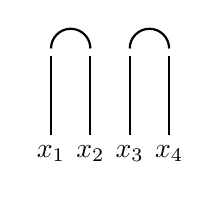
\begin{tikzpicture}[scale=.5, baseline=4mm]
      % lines
      \draw[thick] (0, 0) node[anchor=north] {$x_1$} -- (0, 2);
      \draw[thick] (1, 0) node[anchor=north] {$x_2$}-- (1, 2);
      \draw[thick] (2, 0) node[anchor=north] {$x_3$} -- (2, 2);
      \draw[thick] (3, 0) node[anchor=north] {$x_4$} -- (3, 2);
      % pairings
      \draw[thick] (0, 2.2) arc (180:0:.5);
      \draw[thick] (2, 2.2) arc (180:0:.5);
    \end{tikzpicture}
    +
    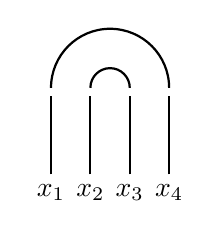
\begin{tikzpicture}[scale=.5, baseline=4mm]
      % lines
      \draw[thick] (0, 0) node[anchor=north] {$x_1$} -- (0, 2);
      \draw[thick] (1, 0) node[anchor=north] {$x_2$}-- (1, 2);
      \draw[thick] (2, 0) node[anchor=north] {$x_3$} -- (2, 2);
      \draw[thick] (3, 0) node[anchor=north] {$x_4$} -- (3, 2);
      % pairings
      \draw[thick] (0, 2.2) arc (180:0:1.5);
      \draw[thick] (1, 2.2) arc (180:0:.5);
    \end{tikzpicture}
    +
    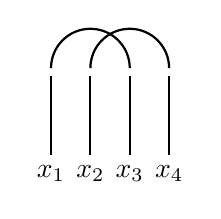
\begin{tikzpicture}[scale=.5, baseline=4mm]
      % lines
      \draw[thick] (0, 0) node[anchor=north] {$x_1$} -- (0, 2);
      \draw[thick] (1, 0) node[anchor=north] {$x_2$}-- (1, 2);
      \draw[thick] (2, 0) node[anchor=north] {$x_3$} -- (2, 2);
      \draw[thick] (3, 0) node[anchor=north] {$x_4$} -- (3, 2);
      % pairings
      \draw[thick] (0, 2.2) arc (180:0:1);
      \draw[thick] (1, 2.2) arc (180:0:1);
    \end{tikzpicture} \\
    &= Q_{12}^{-1} Q_{34}^{-1} + Q_{14}^{-1} Q_{23}^{-1} + Q_{13}^{-1} Q_{24}^{-1}.
  \end{align*}
  On the other hand, for the monomial $\psi = x^4$ there is further symmetry, so we get
  \begin{equation*}
    \avg{x^4} = 3 Q_{11}^{-1} Q_{11}^{-1}.
  \end{equation*}
\end{example}

For a general finite-dimensional vector space $V$ the expectation value corresponds to a map
\begin{equation*}
  \avg{\cdot} \colon \Trm V^\vee \longrightarrow \Rbb
\end{equation*}
where $\Trm V^\vee$ denotes the tensor algebra of $V$. Picking a top form $\mu$ on $V$ we can write
\begin{align*}
  \avg{\phi_{i_1} \otimes \dots \otimes \phi_{i_{2m}}}
  &= \frac{
    \int_V \mu \euler^{-\frac{1}{2} Q(x, x)} \phi_{i_1}(x) \dots \phi_{i_{2m}}(x)
  }{
    \int_V \mu \euler^{-\frac{1}{2} Q(x, x)}
  } \\
  &= \sum_{[\sigma]} (Q^{-1})^{\otimes m} \circ \sigma \circ (\phi_{i_1} \otimes \dots \otimes \phi_{i_{2m}})
\end{align*}

The graphical representation systematize the computations. In this context, a \textbf{graph} consists of:
\begin{enumerate}[i)]
  \item a finite set $V$ of \textbf{vertices};
  \item a finite set $HE$ of \textbf{half-edges} (an even number of them);
  \item an \textbf{incidence} map $i: HE \to V$;
  \item a \textbf{matching} $\sigma$ on $HE$.
\end{enumerate}
A graph automorphism permutes vertices and half-edges, respecting $i$ and $\sigma$.

\begin{example}
  The following graph has a nontrivial automorphism
  \begin{equation*}
    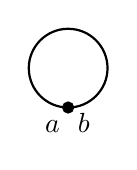
\begin{tikzpicture}
      \draw[fill=black] (0, 0) circle (2pt);
      \draw[thick] (0, .5) circle (5mm);
      \node at (-.2, -.24) {$a$};
      \node at (.2, -.2) {$b$};
    \end{tikzpicture}
  \end{equation*}
  corresponding to permuting half-edges $a \leftrightarrow b$.
\end{example}

\subsection{Expectation value of symmetric tensors}

Consider homogeneous elements $\Psi_1, \dots, \Psi_r \in \Sym V^\vee$ such that
\begin{equation*}
  \Psi_a = \sum (\psi_a)_{i_1, \dots, i_{d_a}} x_{i_1} \dots x_{i_{d_a}}
\end{equation*}
where $|\Psi_a| = d_a$ and $2m = \sum_{a = 1}^r d_a$. We compute the expectation value
\begin{equation*}
  \avg{\Psi_1 \otimes \dots \otimes \Psi_r}
  = \sum_{[\sigma]} (Q^{-1})^{\otimes m} \circ \sigma \circ (\Psi_1 \otimes \dots \otimes \Psi_r ).
\end{equation*}
\begin{example}
  For $\Psi \in \Sym^4 V^\vee$ we have
  \begin{equation*}
    \avg{\Psi}
    =
    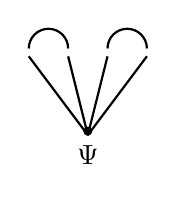
\begin{tikzpicture}[scale=.5, baseline=4mm]
      % node
      \draw[fill=black] (1.5, .1) circle (1mm);
      % lines
      \draw[thick] (1.5, 0) node[anchor=north] {$\Psi$} -- (0, 2);
      \draw[thick] (1.5, 0) -- (1, 2);
      \draw[thick] (1.5, 0) -- (2, 2);
      \draw[thick] (1.5, 0) -- (3, 2);
      % pairings
      \draw[thick] (0, 2.2) arc (180:0:.5);
      \draw[thick] (2, 2.2) arc (180:0:.5);
    \end{tikzpicture}
    +
    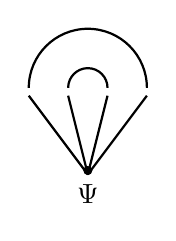
\begin{tikzpicture}[scale=.5, baseline=4mm]
      % node
      \draw[fill=black] (1.5, .1) circle (1mm);
      % lines
      \draw[thick] (1.5, 0) node[anchor=north] {$\Psi$} -- (0, 2);
      \draw[thick] (1.5, 0) -- (1, 2);
      \draw[thick] (1.5, 0) -- (2, 2);
      \draw[thick] (1.5, 0) -- (3, 2);
      % pairings
      \draw[thick] (0, 2.2) arc (180:0:1.5);
      \draw[thick] (1, 2.2) arc (180:0:.5);
    \end{tikzpicture}
    +
    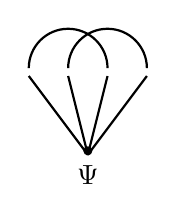
\begin{tikzpicture}[scale=.5, baseline=4mm]
      % node
      \draw[fill=black] (1.5, .1) circle (1mm);
      % lines
      \draw[thick] (1.5, 0) node[anchor=north] {$\Psi$} -- (0, 2);
      \draw[thick] (1.5, 0) -- (1, 2);
      \draw[thick] (1.5, 0) -- (2, 2);
      \draw[thick] (1.5, 0) -- (3, 2);
      % pairings
      \draw[thick] (0, 2.2) arc (180:0:1);
      \draw[thick] (1, 2.2) arc (180:0:1);
    \end{tikzpicture}
    = 3
    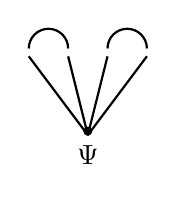
\begin{tikzpicture}[scale=.5, baseline=4mm]
      % node
      \draw[fill=black] (1.5, .1) circle (1mm);
      % lines
      \draw[thick] (1.5, 0) node[anchor=north] {$\Psi$} -- (0, 2);
      \draw[thick] (1.5, 0) -- (1, 2);
      \draw[thick] (1.5, 0) -- (2, 2);
      \draw[thick] (1.5, 0) -- (3, 2);
      % pairings
      \draw[thick] (0, 2.2) arc (180:0:.5);
      \draw[thick] (2, 2.2) arc (180:0:.5);
    \end{tikzpicture}
  \end{equation*}
\end{example}

In general, on $ \avg{ \Psi_1 \otimes \dots \otimes \Psi_r }$ there exists an action of
\begin{equation*}
  S_{d_1} \times \dots \times S_{d_r}
\end{equation*}
therefore we can write
\begin{equation*}
  \bigavg{\frac{1}{d_1!} \Psi_1 \otimes \dots \otimes \frac{1}{d_r!} \Psi_r}
  = \sum_{[\sigma]} \frac{1}{\bigl| \Stab_{[\sigma]} \bigr|}
  (Q^{-1})^{\otimes m} \circ \sigma \circ (\Psi_1 \otimes \dots \otimes \Psi_r)
\end{equation*}
where
\begin{equation*}
  [\sigma] \in \lbigslant{\bigl( \prod_{a = 1}^r S_{d_a} \bigr)}{\text{Matchings}_{2m}}.
\end{equation*}

\begin{example}
  Employing the previous formula we see that
  \begin{equation*}
    \bigavg{\frac{1}{4!} \Psi} = \frac{1}{\bigl| \Stab_{[\sigma]} \bigr|}
    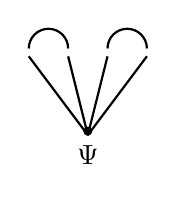
\begin{tikzpicture}[scale=.5, baseline=4mm]
      % node
      \draw[fill=black] (1.5, .1) circle (1mm);
      % lines
      \draw[thick] (1.5, 0) node[anchor=north] {$\Psi$} -- (0, 2);
      \draw[thick] (1.5, 0) -- (1, 2);
      \draw[thick] (1.5, 0) -- (2, 2);
      \draw[thick] (1.5, 0) -- (3, 2);
      % pairings
      \draw[thick] (0, 2.2) arc (180:0:.5);
      \draw[thick] (2, 2.2) arc (180:0:.5);
    \end{tikzpicture}
    = \frac{1}{8} \sum_{i, j, k, l} \Psi_{ijkl} (Q^{-1})_{ik} (Q^{-1})_{jl}.
  \end{equation*}
\end{example}

\begin{example}
  Let $\Psi_1, \Psi_2 \in \Sym^3 V^\vee$. We can verify the previous formula by explicitly computing
  \begin{align*}
    \avg{\Psi_1 \Psi_2}
    &=
    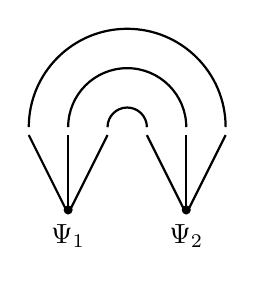
\begin{tikzpicture}[scale=.5, baseline=4mm]
      % nodes
      \draw[fill=black] (1, .1) circle (1mm);
      \draw[fill=black] (4, .1) circle (1mm);
      % lines
      \draw[thick] (1, 0) node[anchor=north] {$\Psi_1$} -- (0, 2);
      \draw[thick] (1, 0) -- (1, 2);
      \draw[thick] (1, 0) -- (2, 2);
      \draw[thick] (4, 0) node[anchor=north] {$\Psi_2$} -- (3, 2);
      \draw[thick] (4, 0) -- (4, 2);
      \draw[thick] (4, 0) -- (5, 2);
      % pairings
      \draw[thick] (0, 2.2) arc (180:0:2.5);
      \draw[thick] (1, 2.2) arc (180:0:1.5);
      \draw[thick] (2, 2.2) arc (180:0:.5);
    \end{tikzpicture}
    + 5 \text{ terms} \\
    &\quad+
    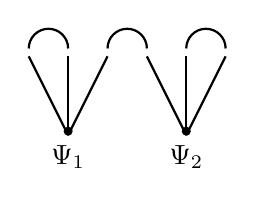
\begin{tikzpicture}[scale=.5, baseline=4mm]
      % nodes
      \draw[fill=black] (1, .1) circle (1mm);
      \draw[fill=black] (4, .1) circle (1mm);
      % lines
      \draw[thick] (1, 0) node[anchor=north] {$\Psi_1$} -- (0, 2);
      \draw[thick] (1, 0) -- (1, 2);
      \draw[thick] (1, 0) -- (2, 2);
      \draw[thick] (4, 0) node[anchor=north] {$\Psi_2$} -- (3, 2);
      \draw[thick] (4, 0) -- (4, 2);
      \draw[thick] (4, 0) -- (5, 2);
      % pairings
      \draw[thick] (0, 2.2) arc (180:0:.5);
      \draw[thick] (2, 2.2) arc (180:0:.5);
      \draw[thick] (4, 2.2) arc (180:0:.5);
    \end{tikzpicture}
    + 9 \text{ terms} \\
    &= 6
    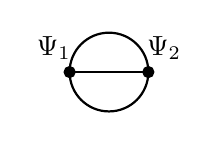
\begin{tikzpicture}[baseline=-1mm]
      % lines
      \draw[thick] (0, 0) node at (-0.2, 0.3) {$\Psi_1$} -- (1, 0) node at (1.2, 0.3) {$\Psi_2$};
      \draw[thick] (0, 0) arc (180:0:.5);
      \draw[thick] (0, 0) arc (-180:0:.5);
      % nodes
      \draw[fill=black] (0, 0) circle (2pt);
      \draw[fill=black] (1, 0) circle (2pt);
    \end{tikzpicture}
    + 9 \ \
    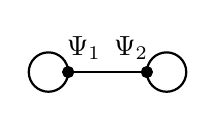
\begin{tikzpicture}[baseline=-1mm]
      % lines
      \draw[thick] (0, 0) node at (0.2, 0.3) {$\Psi_1$} -- (1, 0) node at (0.8, .3) {$\Psi_2$};
      \draw[thick] (-.25, 0) circle (2.5mm);
      \draw[thick] (1.25, 0) circle (2.5mm);
      % nodes
      \draw[fill=black] (0, 0) circle (2pt);
      \draw[fill=black] (1, 0) circle (2pt);
    \end{tikzpicture} \\
    &= \frac{3!3!}{3!}
    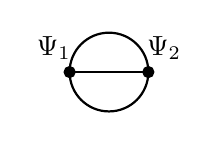
\begin{tikzpicture}[baseline=-1mm]
      % lines
      \draw[thick] (0, 0) node at (-0.2, 0.3) {$\Psi_1$} -- (1, 0) node at (1.2, 0.3) {$\Psi_2$};
      \draw[thick] (0, 0) arc (180:0:.5);
      \draw[thick] (0, 0) arc (-180:0:.5);
      % nodes
      \draw[fill=black] (0, 0) circle (2pt);
      \draw[fill=black] (1, 0) circle (2pt);
    \end{tikzpicture}
    + \frac{3! 3!}{4} \ \
    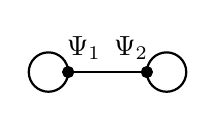
\begin{tikzpicture}[baseline=-1mm]
      % lines
      \draw[thick] (0, 0) node at (0.2, 0.3) {$\Psi_1$} -- (1, 0) node at (0.8, .3) {$\Psi_2$};
      \draw[thick] (-.25, 0) circle (2.5mm);
      \draw[thick] (1.25, 0) circle (2.5mm);
      % nodes
      \draw[fill=black] (0, 0) circle (2pt);
      \draw[fill=black] (1, 0) circle (2pt);
    \end{tikzpicture}.
  \end{align*}
\end{example}

\begin{example}
  The example $\Psi \in \Sym^3 V^\vee$ exhibits more symmetry. As before, we have
  \begin{equation*}
    \avg{\Psi \otimes \Psi}
    = 6
    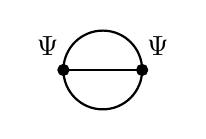
\begin{tikzpicture}[baseline=-1mm]
      % lines
      \draw[thick] (0, 0) node at (-0.2, 0.3) {$\Psi$} -- (1, 0) node at (1.2, 0.3) {$\Psi$};
      \draw[thick] (0, 0) arc (180:0:.5);
      \draw[thick] (0, 0) arc (-180:0:.5);
      % nodes
      \draw[fill=black] (0, 0) circle (2pt);
      \draw[fill=black] (1, 0) circle (2pt);
    \end{tikzpicture}
    + 9 \ \
    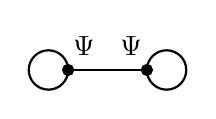
\begin{tikzpicture}[baseline=-1mm]
      % lines
      \draw[thick] (0, 0) node at (0.2, 0.3) {$\Psi$} -- (1, 0) node at (0.8, .3) {$\Psi$};
      \draw[thick] (-.25, 0) circle (2.5mm);
      \draw[thick] (1.25, 0) circle (2.5mm);
      % nodes
      \draw[fill=black] (0, 0) circle (2pt);
      \draw[fill=black] (1, 0) circle (2pt);
    \end{tikzpicture}.
  \end{equation*}
  In this case, there exists an action of $(S_3 \times S_3) \ltimes S_2$ therefore
  \begin{equation*}
    \avg{\Psi \otimes \Psi}
    = \frac{3! 3! 2}{\underbrace{3! 2}_{| \Aut \Lambda |}}
    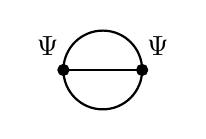
\begin{tikzpicture}[baseline=-1mm]
      % lines
      \draw[thick] (0, 0) node at (-0.2, 0.3) {$\Psi$} -- (1, 0) node at (1.2, 0.3) {$\Psi$};
      \draw[thick] (0, 0) arc (180:0:.5);
      \draw[thick] (0, 0) arc (-180:0:.5);
      % nodes
      \draw[fill=black] (0, 0) circle (2pt);
      \draw[fill=black] (1, 0) circle (2pt);
    \end{tikzpicture}
    + \frac{3! 3! 2}{\underbrace{8}_{|\Aut \Gamma|}} \ \
    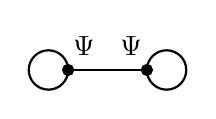
\begin{tikzpicture}[baseline=-1mm]
      % lines
      \draw[thick] (0, 0) node at (0.2, 0.3) {$\Psi$} -- (1, 0) node at (0.8, .3) {$\Psi$};
      \draw[thick] (-.25, 0) circle (2.5mm);
      \draw[thick] (1.25, 0) circle (2.5mm);
      % nodes
      \draw[fill=black] (0, 0) circle (2pt);
      \draw[fill=black] (1, 0) circle (2pt);
    \end{tikzpicture}
  \end{equation*}
  where we identify the denominators with number of automorphisms of the respective graph.
\end{example}

Denote by $\mathsf{Graphs}_{v_0, \dots, v_D}$ the graphs with $v_d$ vertices of valency $0 \leq d \leq D$, where $2m = |HE| = \sum_{d = 0}^D d {v_d}$. There exists a group action
\begin{equation*}
  \prod_{d = 0}^D (S_d)^{v_d} \ltimes S_{v_d} \acts \text{Matchings}_{2m}
\end{equation*}
with what corresponds to graph isomorphisms.

\chapter{Lecture 9 - Manuel Araújo}

\section{Feynman Integrals - Part 2}

% ── Groupoid of graphs ────────────────────────────────────────────────
\subsection{Groupoid of graphs with prescribed vertices}

Let $V_d$ be the set of vertices with valency $d \in \Zbb_{>0}$.
The groupoid $\mathrm{Graphs}_{V_1, \dots, V_D}$ consists of the data:
\begin{itemize}
  \item \textbf{objects:} matchings in HE (set of half-edges);
  \item \textbf{isomorphisms:} collections of morphisms
    \begin{equation*}
      \varphi_d \colon V_d \longrightarrow V_d, \qquad 0 \leq d \leq D
    \end{equation*}
    and $\varphi \colon HE \to HE$ respecting the incidence maps.
\end{itemize}

The action of the group
\begin{equation*}
  G = \prod_{d = 0}^D
  \underbrace{(S_d)^{V_d}}_{\substack{
      \text{permute} \\ \text{half-edges}
  }} \ltimes 
  \underbrace{S_{V_d}}_{\substack{
      \text{permute} \\ \text{vertices}
  }}
\end{equation*}
on $\text{Matchings}_{2m}$ is such that
\begin{equation*}
  \Stab_\sigma \cong \Aut \Gamma_\sigma, \qquad \forall \sigma \in \lbigslant{G}{\text{Matchings}_{2m}}
\end{equation*}
where $\Gamma_\sigma$ is the graph corresponding to a matching $\sigma$, in the obvious way.
Fixing $g \in G$ and $\sigma \in \Mrm_{2m}$ defines a \textit{canonical} isomorphism
\begin{equation*}
  \Gamma_\sigma \longrightarrow \Gamma_{g \cdot \sigma}
\end{equation*}
and we identify $\mathsf{Graphs}_{V_0, \dots, V_D}$ with the \textit{action groupoid} of $G$ acting on $\text{Matchings}_{2m}$.

\begin{example}
  There is an isomorphism of graphs
  \begin{equation*}
    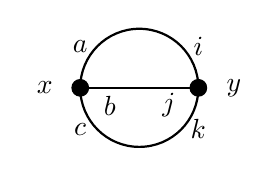
\begin{tikzpicture}[scale = 1.5, baseline=-1mm]
      % lines
      \draw[thick] (0, 0) node at (-.3, 0) {$x$} -- (1, 0) node at (1.3, 0) {$y$};
      \draw[thick] (0, 0) arc (180:0:.5);
      \draw[thick] (0, 0) arc (-180:0:.5);
      % nodes
      \draw[fill=black] (0, 0) circle (2pt);
      \draw[fill=black] (1, 0) circle (2pt);
      \node at (0, .35) {$a$};
      \node at (.25, -.15) {$b$};
      \node at (0, -.35) {$c$};
      \node at (1, .35) {$i$};
      \node at (0.75, -.15) {$j$};
      \node at (1, -.35) {$k$};
    \end{tikzpicture}
    \qquad \underset{
      \begin{aligned}
        i &\mapsto j \\ 
        j &\mapsto i
      \end{aligned}
      }{\cong} \qquad
    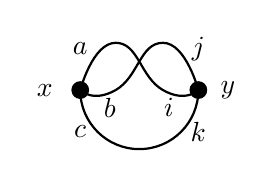
\begin{tikzpicture}[scale = 1.5, baseline=-1mm]
      % lines
      \draw[thick] plot[smooth, tension=1] coordinates { (0, 0) (.3, 0) (.7, .4) (1, 0) };
      \draw[thick] plot[smooth, tension=1] coordinates { (0, 0) (.3, .4) (.7, 0) (1, 0) };
      \draw[thick] (0, 0) arc (-180:0:.5);
      % nodes
      \draw[fill=black] (0, 0) circle (2pt);
      \draw[fill=black] (1, 0) circle (2pt);
      \node at (-.3, 0) {$x$};
      \node at (1.25, 0) {$y$};
      \node at (0, .35) {$a$};
      \node at (.25, -.15) {$b$};
      \node at (0, -.35) {$c$};
      \node at (1, .35) {$j$};
      \node at (0.75, -.15) {$i$};
      \node at (1, -.35) {$k$};
    \end{tikzpicture}
  \end{equation*}
  but no such graph isomorphism exists for between the following graphs.
  \begin{equation*}
  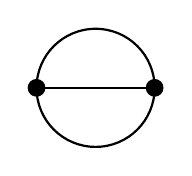
\begin{tikzpicture}[scale = 1.5, baseline=-1mm]
    % lines
    \draw[thick] (0, 0) -- (1, 0);
    \draw[thick] (0, 0) arc (180:0:.5);
    \draw[thick] (0, 0) arc (-180:0:.5);
    % nodes
    \draw[fill=black] (0, 0) circle (2pt);
    \draw[fill=black] (1, 0) circle (2pt);
  \end{tikzpicture}
  \qquad \ncong \qquad
  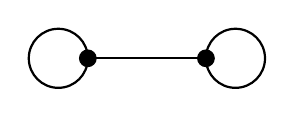
\begin{tikzpicture}[scale =1.5, baseline=-1mm]
    % lines
    \draw[thick] (0, 0) -- (1, 0);
    \draw[thick] (-.25, 0) circle (2.5mm);
    \draw[thick] (1.25, 0) circle (2.5mm);
    % nodes
    \draw[fill=black] (0, 0) circle (2pt);
    \draw[fill=black] (1, 0) circle (2pt);
  \end{tikzpicture}
  \end{equation*}
\end{example}

\begin{example}
  Consider homogeneous polynomials $P_d \in \Sym^d V^\vee$. We compute
  \begin{equation*}
    \bigavg{P_0(x)^{V_0} \dots P_D(x)^{V_D}}
    = \sum_{[\sigma]} \frac{|G|}{|\Aut \Gamma_\sigma|}
    (Q^{-1})^{\otimes m} \circ \sigma \circ (P_0^{V_0} \otimes \dots \otimes P_D^{V_D}) 
  \end{equation*}
  where
  \begin{equation*}
    |G| = \prod_{d = 0}^D (d!)^{V_d} V_d!.
  \end{equation*}
  We can rewrite this as
  \begin{equation*}
    \bigavg{P_0(x)^{V_0} \dots P_D(x)^{V_D}}
    = \biggl( \prod_{d = 0}^D (d!)^{V_d} V_d! \biggr)
    \sum_{\Gamma} \frac{1}{|\Aut \Gamma|} \Phi_{Q^{-1}, \{P_d\}} (\Gamma)
  \end{equation*}
  where we relabel the sum as being over graphs, to which we apply the following procedure.
  \begin{equation*}
    \begin{tikzcd}[sep=small]
    & \Phi_{Q^{-1}, \{{P_d}\}_{d = 0}^D} (\Gamma) \arrow[dr] \arrow[dl] & \\
      \text{label vertices } P_d \arrow[dr] & & \text{label edges } Q^{-1} \arrow[dl] \\
    & \text{contract} &
  \end{tikzcd}
  \end{equation*}
\end{example}

\begin{example}
  For $\Psi \in \Sym^2 V^\vee$ we check that
  \begin{equation*}
    \bigavg{\Psi^3}
    = 8 \cdot 3! \biggl(
      \frac{1}{8 \cdot 3!} \hspace{-4mm}
      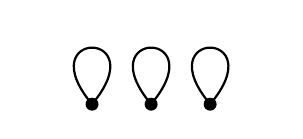
\begin{tikzpicture}[scale=2.5, baseline=2mm]
        % node
        \draw[fill=black] (0, 0) circle (.3mm);
        \draw[fill=black] (.3, 0) circle (.3mm);
        \draw[fill=black] (.6, 0) circle (.3mm);
        % lines
        \draw[thick] (0, 0) to[out=50, in=130, loop] (0, 0);
        \draw[thick] (.3, 0) to[out=50, in=130, loop] (.3, 0);
        \draw[thick] (.6, 0) to[out=50, in=130, loop] (.6, 0);
      \end{tikzpicture}
      \hspace{-4mm} + \frac{1}{8} \hspace{-3mm}
      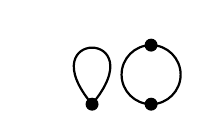
\begin{tikzpicture}[scale=2.5, baseline=2mm]
        % node
        \draw[fill=black] (0, 0) circle (.3mm);
        \draw[fill=black] (.3, 0) circle (.3mm);
        \draw[fill=black] (.3, .3) circle (.3mm);
        % lines
        \draw[thick] (0, 0) to[out=50, in=130, loop] (0, 0);
        \draw[thick] (.3, .15) circle (1.5mm);
      \end{tikzpicture}
      \hspace{1mm} + \frac{1}{6} \hspace{1mm}
      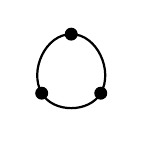
\begin{tikzpicture}[scale=2.5, baseline=2mm]
        % node
        \draw[fill=black] (0, 0) circle (.3mm);
        \draw[fill=black] (.3, 0) circle (.3mm);
        \draw[fill=black] (.15, .3) circle (.3mm);
        % lines
        \draw[thick] (0, 0) to[out=120, in=180] (.15, .3);
        \draw[thick] (.15, .3) to[out=0, in=60] (.3, 0);
        \draw[thick] (0, 0) to[out=-60, in=240] (.3, 0);
      \end{tikzpicture}
    \biggr).
  \end{equation*}
\end{example}

% ── Perturbed Gaussian ────────────────────────────────────────────────
\subsection{Perturbed Gaussian}

We define a \textbf{perturbed} Gaussian integral
\begin{equation*}
  \int_{\Rbb^n}^\text{pert} \drm x \euler^{-\frac{1}{2} Q(x, x) + p(x)}
  = \biggl( \int_{\Rbb^n}^\text{pert} \drm x \euler^{\frac{1}{2} Q(x, x)} \biggr) \bigavg{\euler^{p(x)}}
\end{equation*}
where
\begin{equation*}
  p(x) = \sum_{d = 0}^D \frac{g_d P_d}{d!}, \qquad P_d \in \Sym^d V^\vee.
\end{equation*}
We write
\begin{equation*}
  \euler^{p(x)} 
  = \prod_{d = 0}^D \euler^{\frac{g_d P_d}{d!}}
  = \sum_{V_0, \dots, V_D} \biggl( \prod_{d = 0}^D \frac{g_d^{V_d}}{V_d! (d!)^{V_d}} \biggr)
  P_0(x)^{V_0} \dots P_D(x)^{V_D}
\end{equation*}
therefore
\begin{align*}
  \bigavg{\euler^{p(x)}}
  &= \sum_{V_0, \dots, V_D} g_0^{V_0} \dots g_D^{V_D}
  \sum_{\Gamma \in \mathsf{Graphs}_{V_0, \dots, V_D}}
  \frac{1}{|\Aut \Gamma|} \Phi_{Q^{-1}, \{P_d\}} (\Gamma) \\
  &= \underbrace{\sum_{\Gamma}}_{\substack{\text{sum over} \\ \text{all graphs}}} \frac{1}{|\Aut \Gamma|}
  \underbrace{\Phi_{Q^{-1}, \{g_d P_d\}}}_{\substack{\text{change labels} \\ P_d \, \mapsto \, g_d P_d}}.
\end{align*}

\begin{example}
  Let
  \begin{equation*}
    Q(x, x) = x^2, \qquad p(x) = \frac{\lambda}{4!} x^4.
  \end{equation*}
  In this case
  \begin{align*}
    I^p (\lambda)
    &= \int_{\Rbb^n}^\text{pert} \drm x \euler^{-\frac{1}{2} x^2 + \frac{\lambda}{4!} x^4} \\
    &= \sqrt{2 \pi} \biggl(
      1 + \frac{1}{8} \hspace{-2mm}
      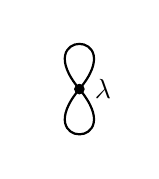
\begin{tikzpicture}[scale=2, baseline=-1mm]
        % node
        \draw[fill=black] (0, 0) circle (.3mm);
        \node at (.15, 0) {$\lambda$};
        % lines
        \draw[thick] (0, 0) to[out=50, in=130, loop] (0, 0);
        \draw[thick] (0, 0) to[out=230, in=-50, loop] (0, 0);
      \end{tikzpicture}
      + \frac{1}{8^2 2} \hspace{-2mm}
      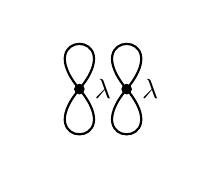
\begin{tikzpicture}[scale=2, baseline=-1mm]
        % node
        \draw[fill=black] (0, 0) circle (.3mm);
        \node at (.15, 0) {$\lambda$};
        \draw[fill=black] (.3, 0) circle (.3mm);
        \node at (.45, 0) {$\lambda$};
        % lines
        \draw[thick] (0, 0) to[out=50, in=130, loop] (0, 0);
        \draw[thick] (0, 0) to[out=230, in=-50, loop] (0, 0);
        \draw[thick] (.3, 0) to[out=50, in=130, loop] (.3, 0);
        \draw[thick] (.3, 0) to[out=230, in=-50, loop] (.3, 0);
      \end{tikzpicture}\\
    &\quad + \frac{1}{4! 2}
      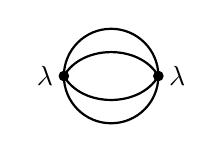
\begin{tikzpicture}[scale=2, baseline=-1mm]
        % node
        \draw[fill=black] (0, 0) circle (.3mm);
        \node at (-.12, 0) {$\lambda$};
        \draw[fill=black] (.6, 0) circle (.3mm);
        \node at (.72, 0) {$\lambda$};
        % lines
        \draw[thick] (.3, 0) circle (3mm);
        \draw[thick] (0, 0) to[out=60, in=120] (.6, 0);
        \draw[thick] (0, 0) to[out=-60, in=-120] (.6, 0);
      \end{tikzpicture}
    + \frac{1}{2^4} 
      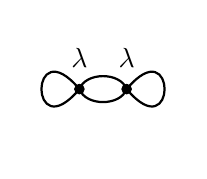
\begin{tikzpicture}[scale=2, baseline=-1mm]
        % node
        \draw[fill=black] (0, 0) circle (.3mm);
        \draw[fill=black] (.3, 0) circle (.3mm);
        \node at (0, .2) {$\lambda$};
        \node at (.3, .2) {$\lambda$};
        % lines
        \draw[thick] (0, 0) to[out=-130, in=130, loop] (0, 0);
        \draw[thick] (.3, 0) to[out=-50, in=50, loop] (.3, 0);
        \draw[thick] (0, 0) to[out=70, in=110] (.3, 0);
        \draw[thick] (0, 0) to[out=-70, in=-110] (.3, 0);
      \end{tikzpicture}
      + \Oscr \bigl(\lambda^3\bigr).
    \biggr) 
  \end{align*}
  The $n$-th coefficient of this series expansion is given by
  \begin{equation*}
    \sum_{\underbrace{\Gamma}_{\substack{n\text{ vertices} \\ \text{of valency } 4}}} \frac{1}{|\Aut \Gamma|}
    = \frac{(4n - 1)!!}{n! 4^n}.
  \end{equation*}
  This expression for $I^p (\lambda)$ has radius of convergence zero. Asymptotically, one can say that for all $N > 0$ there exists $M_N$ such that
  \begin{equation*}
    \biggl| I^p(\lambda) - \sqrt{2 \pi} \sum_{n=0}^N \lambda^n \frac{(4n - 1)!!}{n! 4^n} \biggr|
    \leq M_N |\lambda|^{N + 1}
  \end{equation*}
  for $\lambda < 0$ provided that $|\lambda|$ is sufficiently small.
\end{example}

% ── Connected graphs ──────────────────────────────────────────────────
\subsection{Connected graphs}

It can be useful to rewrite the usual expression in term of connected graphs. To achieve this, we decompose the sum with respect to the number of connected components of the graphs
\begin{align*}
  \sum_{\Gamma} \frac{1}{|\Aut \Gamma|} \Phi(\Gamma)
  &= \overbrace{\sum_{k = 0}^\infty}^{\substack{\text{connected}\\ \text{components}}}
  \sum_{\gamma_1, \dots, \gamma_k}
  \overbrace{\sum_{r_1, \dots, r_k = 1}^\infty}^{\text{valencies}}
  \biggl( \prod_{i=1}^k \frac{1}{r_i! |\Aut \gamma_i|} \biggr) \Phi(\gamma_1)^{r_1} \dots \Phi(\gamma_k)^{r_k} \\
  &= \underbrace{\prod_{\gamma \text{ connected}}}_{\substack{\text{finitely-many} \\ \text{nonzero valencies}}}
    \biggl( \sum_{r=0}^\infty \frac{1}{r! |\Aut \gamma|^r} \Phi(\gamma)^r \biggr) \\
  &= \prod_{\gamma \text{ connected}} \exp \biggl( \frac{1}{|\Aut \gamma|} \Phi(\gamma) \biggr) \\
  &= \exp \Biggl( \sum_{\gamma \text{ connected}} \frac{1}{|\Aut \gamma|} \Phi(\gamma) \Biggr).
\end{align*}

\chapter{Lecture 10}

\section{Scalar QFT in the Wilsonian Sense}

The main reference for this lecture is \cite[Sections 1.1 to 1.5 and 2.1 to 2.7]{CosRenormalization11}.
Our goal is to give a Wilsonian definition of scaler QFT. Consider the data:
\begin{enumerate}[i)]
  \item \textbf{spacetime:} smooth Riemannian manifold $M$ (we consider $M = \Rbb^n$);
  \item \textbf{scalar fields:} smooth functions $ \varphi \colon M \to \Rbb$;
  \item \textbf{action functional:} a local functional
  \begin{equation*}
    S(\varphi) = \int_M - \frac{1}{2} \varphi \bigl( \Drm + m^2 \bigr) \varphi 
    + \hspace{-7mm} \underbrace{I (\varphi)}_{\substack{
        \text{interactions terms} \\
        \text{(cubic or higher)}}}
  \end{equation*}
  where we call $m > 0$ the \textit{mass parameter} and $\Drm$ denotes the Laplacian.
\end{enumerate}

For the Dirichlet problem on some domain $U \subseteq M$
\begin{equation*}
  \begin{cases}
    \Drm \varphi(x) + \lambda \varphi(x), &\text{ if } x \in U \\
    \varphi(x) = 0, &\text{ if } x \in \partial U
  \end{cases}
\end{equation*}
we write the associated eigenfunctions $\varphi_n$ with corresponding eigenvalues $\lambda_n$.
It is known that the inverse Laplacian operator is compact and self-adjoint. From the spectral theorem follows that
\begin{equation*}
  0 < 
  \underbrace{\lambda_1 \leq \dots \leq \lambda_n}_{\text{energies}}
  \leq \dots \longrightarrow \infty.
\end{equation*}

In this context, \textbf{observables} are functionals $\Ocal : \Crm^\infty (M) \to \Cbb$.

\begin{example}
  The evaluation map is an observable
  \begin{equation*}
    \Ocal_x (\varphi) = \varphi(x), \quad \forall x \in M.
  \end{equation*}
\end{example}

The physical information of the theory is encoded in the correlation functions, which we compute (up to normalization) using the Feynman sum of histories approach
\begin{equation*}
  \langle \Ocal_1, \dots, \Ocal_n \rangle
  = \int_{\varphi \in \Crm^\infty(M)} \euler^{\frac{1}{\hbar} S(\varphi) }
  \Ocal_1(\varphi) \dots \Ocal_n(\varphi) \Drm \varphi.
\end{equation*}

To proceed, we restrict to \textit{low-energy fields}
\begin{equation*}
  \Crm_{\leq \Lambda} = \Crm^\infty(M)_{\leq \Lambda}
\end{equation*}
corresponding to the space spanned by eigenfunctions with associated energy $\lambda_n \leq \Lambda$ (in principle finite-dimensional), and \textit{low-energy observables}
\begin{equation*}
  (\Ocal \colon \Crm_{\leq \Lambda} \longrightarrow \Cbb) \in \Obs_{\leq \Lambda}.
\end{equation*}
Then
\begin{equation*}
  \langle \Ocal_1, \dots, \Ocal_n \rangle
  = \int_{\varphi \in \Crm_{\leq \Lambda}}
  \euler^{\frac{1}{\hbar} S^\text{eff}[\Lambda](\varphi)} \Ocal_1 (\varphi) \dots \Ocal_n (\varphi) \Drm \varphi
\end{equation*}
for some low-energy \textbf{effective action} $S^\text{eff}[\Lambda]$. For low-energy observable we have
\begin{equation*}
  \Ocal \in \Obs_{\leq \Lambda'} \Longrightarrow
  \Ocal \in \Obs_{\leq \Lambda}, \quad 0 < \Lambda' < \Lambda
\end{equation*}
which motivates the decomposition of fields into \textit{low-} and \textit{high-energy} parts
\begin{equation*}
  \varphi = \varphi_L + \varphi_H, \quad \varphi_L \perp \varphi_H
\end{equation*}
where $\varphi_L$ is the projection of $\varphi$ on $\Crm_{\leq \Lambda'}$, and $\varphi_H$ the corresponding parallel component in $\Crm_{\leq \Lambda}$. Then
\begin{align*}
  &\quad \int_{\varphi_L \in \Crm_{\leq \Lambda'}} \euler^{\frac{1}{\hbar} S^\text{eff} [\Lambda'] (\varphi_L)}
    \Ocal_1 (\varphi_L) \dots \Ocal_n (\varphi_L) \Drm \varphi \\
  &= \int_{\varphi \in \Crm_{\leq \Lambda}} \euler^{\frac{1}{\hbar} S^\text{eff}[\Lambda](\varphi)}
    \Ocal_1 (\varphi) \dots \Ocal_n(\varphi) \Drm \varphi \\
  &= \int_{\varphi_L} 
  \biggl(\int_{\varphi_H} \euler^{\frac{1}{\hbar} S^\text{eff}[\Lambda] (\varphi_L+\varphi_H)}\biggr)
  \Ocal_1(\varphi_L) \dots \Ocal_n (\varphi_L) \Drm \varphi
\end{align*}
implying that
\begin{equation*}
  \euler^{\frac{1}{\hbar} S^\text{eff}[\Lambda'] (\varphi_L)}
  = \int_{\varphi_H} \euler^{\frac{1}{\hbar} S^\text{eff} [\Lambda] (\varphi_L + \varphi_H)} \Drm \varphi_H.
\end{equation*}
Taking the logarithm we obtain the \textbf{renormalization group equation} (RGE)
\begin{equation*}
  S^\text{eff}[\Lambda'] (\varphi_L)
  = \hbar \log \int_{\varphi_H} \euler^{\frac{1}{\hbar} S^\text{eff}[\Lambda] (\varphi_L + \varphi_H)} 
  \Drm \varphi_H.
\end{equation*}

\subsection{Renormalization Group Equation}

Assume that
\begin{equation*}
  S^\text{eff}[\Lambda] (\varphi) = \int_M - \frac{1}{2} \varphi \bigl(D + m^2\bigr) \varphi
  + \hspace{-3mm}
  \underbrace{I^\text{eff}[\Lambda] (\varphi)}_{\text{effective interaction}} \hspace{-2mm}.
\end{equation*}
From the linearity of the Laplacian and the RGE follows that
\begin{equation*}
  I^\text{eff}[\Lambda'](\varphi_L)
  = \hbar \log \int_{\varphi_H} \exp
    \biggl( -\frac{1}{2 \hbar} \varphi_H \bigl(D + m^2\bigr) \varphi_H
    + \frac{1}{\hbar} I^\text{eff}[\Lambda] (\varphi_L + \varphi_H) \biggr) \Drm \varphi_H.
\end{equation*}

We are interested in finite-dimensional integrals of the form
\begin{equation*}
  W(P, I)
  = \int_U \exp \biggl( 
    \frac{1}{2 \hbar} \Phi (x, x)
    + \frac{1}{\hbar} I(x + a)
  \biggr) 
\end{equation*}
for some nondegenerate negative-definite quadratic form $\Phi$, understood as a Feynman diagram expansion.
Here $P$ is the integral kernel of $(\Drm + m^2)^{-1}$ (propagator)
\begin{equation*}
  P(x, y) = \int_{\tau = 0}^\infty \euler^{-\tau m^2} \dd \tau
  \underbrace{K_\tau^0 (x, y)}_{\text{heat kernel}}
\end{equation*}
where we write
\begin{equation*}
  K_\tau^0 (x, y)
  = \int_{f \in \Omega_{x, y}}
  \exp \biggl( \int_0^\tau \| \drm f \|^2 \dd s \biggr) \dd W
\end{equation*}
for
\begin{equation*}
  \Omega_{x, y} = \{
    f : [0, \tau] \to M \mid f(0) = x, f(\tau) = y
  \}.
\end{equation*}
In terms of eigenfunctions
\begin{equation*}
  K_\tau^0 (x, y) 
  = \sum_{n=0}^\infty \euler^{-\lambda_n \tau}
  \varphi_n (x) \varphi_n (y)
\end{equation*}
and $K_\tau = K_\tau^0 \euler^{\tau m^2}$ is such that
\begin{equation*}
  P(x, y) = \int_{\tau = 0}^\infty K_\tau (x, y) \dd \tau.
\end{equation*}

\subsection{Length scale instead of energy scale}

The high-energy regimes correspond to small scales:
\begin{equation*}
  \text{short lengths} \leftrightsquigarrow
  \text{high energy}.
\end{equation*}
Because of this, the RGE should relate different length scales
\begin{equation*}
  P(\varepsilon, L) (x, y)
  = \int_{l=\varepsilon}^{L} K_l(x, y) \dd l.
\end{equation*}
Again, the RGE for relating different scales
\begin{equation*}
  I^\text{eff}[L] = W\bigl(P(\varepsilon, L), I^\text{eff}[\varepsilon]\bigr)
\end{equation*}
is given in terms of Feynman diagrams.
Expanding in powers
\begin{equation*}
  I^\text{eff} = \sum_{i, j} \hbar^j \varphi^k I_{j, k}.
\end{equation*}

\begin{example}
  Some examples of the diagrammatic approach are
  \begin{equation*}
    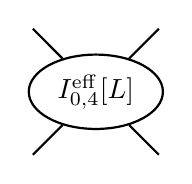
\begin{tikzpicture}[scale=0.8, baseline=-1mm]
      \node[ellipse, draw, thick] (A) at (0, 0) {$I_{0, 4}^\text{eff} [L]$};
      \draw[thick] (A) -- (1, 1);
      \draw[thick] (A) -- (1, -1);
      \draw[thick] (A) -- (-1, 1);
      \draw[thick] (A) -- (-1, -1);
    \end{tikzpicture}
    \hspace{3mm}= \hspace{3mm}
    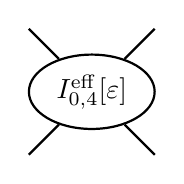
\begin{tikzpicture}[scale=0.8, baseline=-1mm]
      \node[ellipse, draw, thick] (A) at (0, 0) {$I_{0, 4}^\text{eff} [\varepsilon]$};
      \draw[thick] (A) -- (1, 1);
      \draw[thick] (A) -- (1, -1);
      \draw[thick] (A) -- (-1, 1);
      \draw[thick] (A) -- (-1, -1);
    \end{tikzpicture}
    \hspace{3mm} +
    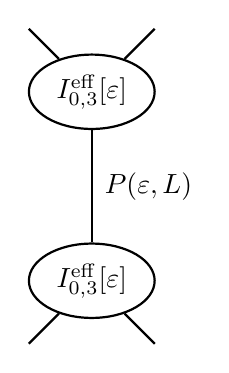
\begin{tikzpicture}[scale=0.8, baseline=-1mm]
      \node[ellipse, draw, thick] (A) at (0, -1.5) {$I_{0, 3}^\text{eff}       [\varepsilon]$};
      \node[ellipse, draw, thick] (B) at (0, 1.5) {$I_{0, 3}^\text{eff}       [\varepsilon]$};
      \draw[thick] (A) -- (1, -2.5);
      \draw[thick] (A) -- (-1, -2.5);
      \draw[thick] (A) -- (B);
      \draw[thick] (B) -- (1, 2.5);
      \draw[thick] (B) -- (-1, 2.5);
      \node at (.9, 0) {$P(\varepsilon, L)$};
    \end{tikzpicture}
  \end{equation*}
  and
  \begin{equation*}
    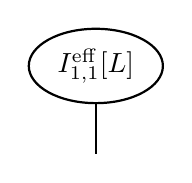
\begin{tikzpicture}[scale=0.8, baseline=-1mm]
      \node[ellipse, draw, thick] (A) at (0, 0) {$I_{1, 1}^\text{eff}       [L]$};
      \draw[thick] (A) -- (0, -1.4);
    \end{tikzpicture}
    \hspace{5mm}=\hspace{5mm}
    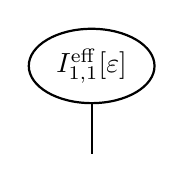
\begin{tikzpicture}[scale=0.8, baseline=-1mm]
      \node[ellipse, draw, thick] (A) at (0, 0) {$I_{1, 1}^\text{eff}       [\varepsilon]$};
      \draw[thick] (A) -- (0, -1.4);
    \end{tikzpicture}
    \hspace{5mm}+ \hspace{5mm}
    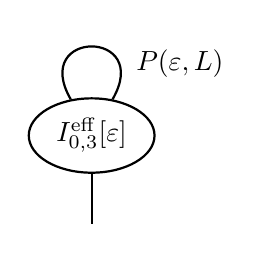
\begin{tikzpicture}[scale=0.8, baseline=-1mm]
      \node[ellipse, draw, thick] (A) at (0, 0) {$I_{0, 3}^\text{eff}       [\varepsilon]$};
      \draw[thick] (A) -- (0, -1.4);
      \draw[thick] (A) to[out=60, in=120, loop, looseness=5] (A);
      \node at (1.4, 1.15) {$P(\varepsilon, L)$};
    \end{tikzpicture}.
  \end{equation*}
\end{example}

\begin{definition}
  A \textbf{perturbative QFT} with space of fields and action functional as prescribed earlier, is given by a set of interactions $I[L]$ such that:
  \begin{enumerate}[i)]
    \item the RGE holds for any positive scales:
      \begin{equation*}
        I[L] = W \bigl(p(\varepsilon, L), I[\varepsilon]\bigr), \qquad
        \forall \varepsilon, L \in (0, \infty];
      \end{equation*}
    \item the components $I_{j, k}$ are \textbf{local:} if
      \begin{equation*}
        S^\text{eff}[L] (\varphi)
        = \sum_{i} f_i (L) \Theta_i (\varphi)
      \end{equation*}
      then $\Theta_i$ are local functionals.
  \end{enumerate}
\end{definition}

\chapter{Lecture 11 - Leander Stecker}

\section{Elliptic Operators and Complexes}

Let $M$ be a closed, oriented Riemannian manifold, and $E, F \to M$ complex vector bundles over $M$.
A \textbf{differential operator}
\begin{equation*}
  P \colon \Gamma (E) \longrightarrow \Gamma(F)
\end{equation*}
is a $\Cbb$-linear map that, in local coordinates $(U, x^i)$ of $M$ with local trivializations of $E$ and $F$, has the form
\begin{equation*}
  P = \sum_{|\alpha| \leq k} A^\alpha
  \frac{\partial^{|\alpha|} }{\partial x^{\alpha}}
\end{equation*}
where $\alpha$ is a multi-index and
\begin{equation*}
  A^\alpha \in \Hom ( E |_U, F |_U )
\end{equation*}
is a bundle map over $U$.
The number $k \in \Zbb_{\geq 0}$ is called the \textbf{order} of $P$.

\begin{definition}
  The \textbf{principal symbol} $\sigma(P)$ of a differential operator is a section of the pullback bundle
  $\pi^* \Hom(E, F)$ over $T^*M$, as in the following diagram.
  \begin{equation*}
    \begin{tikzcd}[sep=large]
      |[label={-45:\lrcorner}]|
      \pi^* \Hom(E, F) \arrow[r] \arrow[d] &
      \Hom(E, F) \arrow[d] \\
      T^* M \arrow[r, "\pi"] &
      M
    \end{tikzcd}
  \end{equation*}
\end{definition}

At $\xi \in T^* M$, $\sigma(P)$ is given by
\begin{equation*}
  \sigma(P)_\xi = \sum_{|\alpha| \leq k} A^\alpha (x) \xi_\alpha
\end{equation*}
where for $\alpha = (\alpha_1, \dots, \alpha_n)$, we write $\xi = \xi_i \drm x^i$.
Since $\sigma(P)$ is the only symbol we will need, let us just call it the \textit{symbol} of $P$.

\begin{lemma}
  The symbol of $P$ is equivalently defined by
  \begin{equation*}
    \sigma(P)_\xi = \lim_{t \to \infty} (it)^{-k} \euler^{-i t f}
    P \euler^{i t f}
  \end{equation*}
  where $f$ is any smooth function such that
  \begin{equation*}
    \drm f (x) = \xi.
  \end{equation*}
\end{lemma}
\begin{proof}
  In a local trivialization over a chart, for a local section $s$, we compute
  \begin{align*}
    P \euler^{i t f} s
     & = \sum_{|\alpha| \leq k} A^\alpha
    \frac{\partial^{|\alpha|}}{\partial x^\alpha}
    \bigl( \euler^{i t f} s \bigr)       \\
     & = \sum_{|\alpha| \leq k} (i t)^k
    \frac{\partial^{|\alpha|} f}{\partial x^\alpha} \euler^{i t f}
    A^\alpha s +
    \substack{\text{lower}               \\ \text{order in } t}
  \end{align*}
  hence
  \begin{equation*}
    \lim_{t \to \infty} (it)^{-k} \euler^{-i t f} P \euler^{i t f} s
    = \sum_{|\alpha| = k} \drm f \biggl( \frac{\partial^|\alpha|}{\partial x^\alpha} \biggr) A^\alpha s.
  \end{equation*}
  Evaluating at $x$ gives $\sigma(P)_\xi$.
\end{proof}

\begin{example}
  The exterior derivative
  \begin{equation*}
    \drm \colon \Omega^\bullet(M) \longrightarrow \Omega^\bullet (M)
  \end{equation*}
  can be writen in local coordinates as
  \begin{equation*}
    \drm = \sum_{i=1}^n \frac{\partial}{\partial x^i} \drm x^i \wedge
  \end{equation*}
  therefore
  \begin{equation*}
    \sigma(\drm)_\xi = \sum_{i=1}^n \xi_i \drm x^i \wedge = \xi \wedge
  \end{equation*}
  so the symbol is given by the wedge product.
\end{example}

\begin{example}
  The Laplacian
  \begin{equation*}
    \laplace \colon \Crm^\infty(M) \longrightarrow \Crm^\infty (M)
  \end{equation*}
  can be writen in normal coordinates around $p \in M$
  \begin{equation*}
    \laplace |_p = - \sum_{i = 1}^n
    \biggl( \frac{\partial}{\partial x^i} \biggr)^2
  \end{equation*}
  hence $\sigma (\laplace)_\xi = - |\xi|^2$.
\end{example}

\begin{example}
  The Hodge Laplacian
  \begin{equation*}
    \laplace \colon \Omega^\bullet (M) \longrightarrow \Omega^\bullet (M)
  \end{equation*}
  is given by
  \begin{align*}
    \laplace
     & = \drm \drm^\hodge + \drm^\hodge \drm                            \\
     & = - \sum_{i=1}^n \biggl( \frac{\partial}{\partial x^i} \biggr)^2
    \Bigl( \iota_{\frac{\partial}{\partial x^i}} \drm x^i
    + \drm x^i \iota_{\frac{\partial}{\partial x^i} }\Bigr)             \\
     & = - \sum_{i=1}^n
    \Bigl[ \iota_{\frac{\partial}{\partial x^i}}, \drm x^i \Bigr]
    \biggl( \frac{\partial}{\partial x^i} \biggr)^2
  \end{align*}
  where $\iota_{\frac{\partial}{\partial x^i}}$ denotes the interior product and $\drm x^i$ is the operator $\drm x^i \wedge$ in $\Omega^\bullet (M)$.

  Remarkably, we still have $\sigma(\laplace)_\xi = - |\xi|^2$. To see this, we need the following proposition.

  \begin{proposition}
    For differential operators $P$ and $P'$ we have
    \begin{equation*}
      \sigma(P)_\xi \sigma(P')_\xi = \sigma(P P')_\xi.
    \end{equation*}
  \end{proposition}
  \begin{proof}
    If $P$ has order $k$ and $P'$ has order $k'$, then $P P'$ has order $k + k'$ and
    \begin{align*}
       & \quad \lim_{t \to \infty}
      \Bigl( (i t)^{-k} \euler^{-i t f} P \euler^{i t f} \Bigr)
      \Bigl( (i t)^{-k'} \euler^{- i t f} P' \euler^{i t f} \Bigr) \\
       & = \lim_{t \to \infty}
      \Bigl( (i t )^{-k-k'} \euler^{- i t f} P P' \euler^{i t f} \Bigr).
    \end{align*}
  \end{proof}

  We also need that
  \begin{equation*}
    \sigma( \drm^\hodge)_\xi = - \iota_{\xi^\#}
  \end{equation*}
  where $\xi^\# \in T_x M$ is the unique vector such that $\xi = g(\xi^\#, \cdot)$. Then
  \begin{align*}
    \sigma(\laplace)_\xi
     & = \sigma(\drm \drm^\hodge + \drm^\hodge \drm)_\xi              \\
     & = \sigma(\drm \drm^\hodge)_\xi + \sigma (\drm^\hodge \drm)_\xi \\
     & = \bigl[\xi, - \iota_{\xi^\#}\bigr]                            \\
     & = - | \xi |^2.
  \end{align*}
\end{example}

\begin{definition}
  An operator $P \colon \Lambda (E) \to \Lambda(F)$ is \textbf{elliptic} if the symbol $\sigma(P)_\xi$ is invertible for all $\xi \neq 0$.
\end{definition}
Remember that, for all $\xi \in T_x^*M$, the symbol is a linear operator $\sigma(P)_\xi \colon E_x \to F_x$.

\begin{definition}
  An operator $P : \Lambda(E) \to \Lambda(E)$ is called a \textbf{generalized Laplacian} if
  \begin{equation*}
    \sigma(P)_\xi = - |\xi|_{\tilde{g}}^2
  \end{equation*}
  for some metric $\tilde{g}$ on $M$, not necessarily the one we started with.
\end{definition}
The previous definition comes from \cite{BGVHeat96}, but we have taken the opposite sign convention.

\section{Elliptic Complexes}

Suppose $P \colon \Gamma(E) \to \Gamma(F)$ is elliptic. The symbol $\sigma(P)$ defines a bundle map over $T^*M$
\begin{equation*}
  \begin{tikzcd}
    0 \arrow[r] &
    \pi^* E \arrow[r, "\sigma(P)"] &
    \pi^* F \arrow[r] & 0
  \end{tikzcd}
\end{equation*}
which is exact over $T^*M$ away from the zero section.
Now let $(E^\bullet, Q)$ be the $\Zbb$-graded vector bundle $E^\bullet \to M$, and
\begin{equation*}
  Q \colon \Gamma(E^\bullet) \longrightarrow \Gamma(E^\bullet)
\end{equation*}
a differential operator of cohomological degree $1$ such that $Q^2 = 0$.

\begin{definition}
  The complex $(E^\bullet, Q)$ is an \textbf{elliptic complex} if the symbol complex $(\pi^* E, \sigma(Q))$ is exact over $T^*M \to M$.
\end{definition}

\begin{example}
  To the de Rham complex
  \begin{equation*}
    \begin{tikzcd}
      0 \arrow[r] &
      \Omega^0 (M) \arrow[r, "\drm"] &
      \Omega^1 (M) \arrow[r, "\drm"] &
      \dots \arrow[r, "\drm"] &
      \Omega^n (M)
    \end{tikzcd}
  \end{equation*}
  corresponds the symbol complex for $\xi \in \Omega^1 (M)$
  \begin{equation*}
    \begin{tikzcd}
      0 \arrow[r] &
      \Omega^0 (M) \arrow[r, "\xi"] &
      \Omega^1 (M) \arrow[r, "\xi"] &
      \dots \arrow[r, "\xi"] &
      \Omega^n (M)
    \end{tikzcd}.
  \end{equation*}
  If $\xi \neq 0$ and $\xi \wedge \beta = 0$, then $\beta = \xi \wedge \alpha$ for some $\alpha \in \Omega^\bullet(M)$. We conclude that the symbol complex is exact, and thus $(\Omega^\bullet, \drm)$ is an elliptic complex.
\end{example}

\begin{example}
  To the Yang-Mills complex
  \begin{equation*}
    \begin{tikzcd}
      \Omega^0(M, \gfrak) \arrow[r, "\drm"] &
      \Omega^1(M, \gfrak) \arrow[r, "\drm \hodge \drm"] &
      \Omega^{n-1} (M, \gfrak) \arrow[r, "\drm"] &
      \Omega^n(M, \gfrak)
    \end{tikzcd}
  \end{equation*}
  we associate
  \begin{equation*}
    \begin{tikzcd}[sep=small]
      0 \arrow[r] &
      \bigwedge^0 (M) \otimes \gfrak \arrow[r] &
      \bigwedge^1 (M) \otimes \gfrak \arrow[r] &
      \bigwedge^{n-1} (M) \otimes \gfrak \arrow[r] &
      \bigwedge^n (M) \otimes \gfrak \arrow[r] & 0
    \end{tikzcd}.
  \end{equation*}
  The de Rham complex is exact, so it suffices to show that
  \begin{equation*}
    \ker \bigl( \sigma(\drm \hodge \drm)_\xi \bigr)
    = \ker (\xi \wedge)
  \end{equation*}
  by showing that
  \begin{equation*}
    \underbrace{\ker \bigl( \sigma(\drm \hodge)_\xi \bigr)}_{\ker(- \iota_\xi)}
    \cap \underbrace{\Image \sigma(\drm)_\xi}_{\Image(\xi \wedge)} = 0.
  \end{equation*}
\end{example}

Suppose that $(E^\bullet, Q)$ is elliptic and choose $h_i$ a Hermitian metric on $E^i$.
Define a $\Lrm^2$-norm on sections
\begin{equation*}
  h_i^{\Lrm^2}(s, s')
  = \int_M h_i (s, s') \dd \text{vol}_g (x).
\end{equation*}
The we a get a \textit{formal adjoint}
\begin{equation*}
  \begin{tikzcd}
    \dots &
    \Ecal^{i-1} \arrow[l, swap, "Q^*"] &
    \Ecal^{i} \arrow[l, swap, "Q^*"] &
    \Ecal^{i+1} \arrow[l, swap, "Q^*"] &
    \dots \arrow[l, swap, "Q^*"]
  \end{tikzcd}
\end{equation*}
defined such that
\begin{equation*}
  h_{i+1}^{\Lrm^2}(Q u, v) = h_i^{\Lrm^2} (u, Q^* v), \qquad
  \forall u \in \Ecal^{i}, \forall v \in \Ecal^{i+1}.
\end{equation*}

\begin{lemma}
  The operator
  \begin{equation*}
    \Drm = [Q, Q^*] = Q Q^* + Q^* Q
  \end{equation*}
  is elliptic.
\end{lemma}
\begin{proof}
  Note that
  \begin{equation*}
    \sigma(Q^*)_{\xi_x} = \bigl( \sigma(Q)_{\xi_x} \bigr)^*
  \end{equation*}
  where the second $*$ denotes the usual finite-dimensional adjoint with respect to the fiber metric.
  Thus,
  \begin{equation*}
    \sigma(\Drm)
    = \sigma(Q) \sigma(Q^*) + \sigma(Q^*) \sigma(Q) \\
    = \sigma(Q) \sigma(Q)^* + \sigma(Q)^* \sigma(Q)
  \end{equation*}
  and for all $v \in \ker \bigl( \sigma(\Drm)_\xi \bigr)$ we have
  \begin{equation*}
    0 = h\bigl(v, \sigma(\Drm)_\xi v \bigr)
    = \bigl| \sigma(Q)_\xi  v \bigr|_h^2 + \bigl| \sigma(Q)_\xi^* v \bigr|_h^2.
  \end{equation*}
  We conclude that
  \begin{equation*}
    v \in \ker \bigl( \sigma(Q)_\xi \bigr) \cap
    \ker \bigl( \sigma(Q)_\xi^* \bigr)
    = \ker \bigl( \sigma(Q)_\xi \bigr) \cap
    \ker \bigl( \sigma(Q)_\xi \bigr)^\perp
  \end{equation*}
  implying that $v = 0$.
\end{proof}

\chapter{Lecture 12 - Leander Stecker}

% ── Gauge Fixing Operator ─────────────────────────────────────────────
\section{Gauge Fixing Operator}

\begin{definition}
  A free theory in the BV formalism is the data:
  \begin{enumerate}[i)]
    \item a $\Zbb$-graded vector bundle $E \to M$;
    \item a Hermitian nondegenerate pairing $\langle \cdot, \cdot \rangle$ of degree $-1$;
    \item a differential operator $Q \colon \Gamma(E) \to \Gamma(E)$ of degree $1$ such that $Q^2 = 0$, $Q$ is skew-symmetric with respect to the pairing, and wields an elliptic complex $(E, Q)$.
  \end{enumerate}
\end{definition}

\begin{definition}
  Let
  $Q^\text{GF} \colon \Gamma(E) \to \Gamma(E)$
  be a differential operator of degree $-1$, symmetric with respect to the pairing $\langle \cdot, \cdot \rangle$.
  This operator is a \textit{generalized Laplacian} if $\Drm = \big[Q, Q^\text{GF}\big]$ is such that
  \begin{equation*}
    \sigma(\Drm)_\xi = - |\xi|^2
  \end{equation*}
  where $|\cdot|$ is defined with respect to any metric on $M$.
  If this condition holds, we say that $Q^\text{GF}$ is a \textit{gauge fixing operator}.
\end{definition}

% ── Heat Kernels and Propagators ──────────────────────────────────────
\section{Heat Kernel and Propagators}

\begin{theorem}
  Fix a Hermitian metric $h^i$ on the fibers $E^i$.
  Suppose that $P$ is an elliptic operator, symmetric and positive, that is
  \begin{equation*}
    h^{\Lrm^2}(P s, s) \geq 0, \qquad \forall s \in \Gamma(E).
  \end{equation*}
  Then:
  \begin{enumerate}[i)]
    \item if $u \in \Hrm^\Srm (M, E)$ for some Sobolev space, and $P u \in \Crm^\infty (M, E)$, then $u \in \Crm^\infty(E, M)$;
    \item there exists a complex orthonormal basis $\{ u_j \}_{j \in \Zbb_{\geq 0}}$ of $\Lrm^2 (M, E)$ consisting of smooth eigensections of $P$, with eigenvalues
          \begin{equation*}
            0 \geq \lambda_1 \geq \dots \geq \lambda_n \geq \dots
          \end{equation*}
          such that $\lambda_j \geq C j^c$, for some $c = c(n, k) > 0$ depending on $n$ and $k$, and $C > 0$.
  \end{enumerate}
\end{theorem}

\begin{proof}
  A \textit{rough idea} of the proof is the following. Inverting the symbol gives a pseudo-differential operator that is homogeneous in $\xi^{-k}$.
  Construct an almost-inverse $P^{-1}$ to $P$.
  This operator smooths out functions, implying the first item.
  The second item is a consequence of the spectral theorem for compact operators.
\end{proof}

The operator $\Drm = P P^* + P^* P$ obeys the conditions of the previous theorem.
A generalized Laplacian is, in general, not symmetric nor positive, only at higher order.
However, a generalized Laplacian is of the form
\begin{equation*}
  \Drm^\nabla + \Frm
\end{equation*}
where $\Drm^\nabla$ is symmetric and positive, and $\Frm$ is of order $0$.


% ── Bibliography ──────────────────────────────────────────────────────
\sloppy
\printbibliography

\end{document}
